%% Beispiel-Präsentation
\documentclass{sdqbeamer}
 
%% Titelbild
\titleimage{banner_2020_kit}

%% Gruppenlogo
\grouplogo{hci}

%% Gruppenname und Breite (Standard: 50 mm)
\groupname{Mensch-Maschine-Interaktion und Barrierefreiheit}
%\groupnamewidth{50mm}

% Beginn der Präsentation

\title[Solidarische Raumnutzung Entwurfsheft]{Kolloquium Entwurfsheft zur Solidarischen Raumnutzung}
\author[Soli-Gruppe]{Alexander Klee, Jannik Hönlinger, Johannes Frohnmeyer, Ben Steinle und Antonia Ammon }
\subtitle{PSE-Projekt WS24/25}
\date[03.\,01.\,2025]{03. Januar 2025}

% Literatur
 
\usepackage[citestyle=authoryear,bibstyle=numeric,hyperref,backend=biber]{biblatex}
\addbibresource{presentation.bib}
\bibhang1em

\begin{document}
 
%Titelseite
\KITtitleframe

%Gliederung
\begin{frame}{Gliederung}
\tableofcontents
\end{frame}

\section{Aufbau}

\subsection{Architektur}
\begin{frame}{Architektur}
\begin{figure}
    \centering
    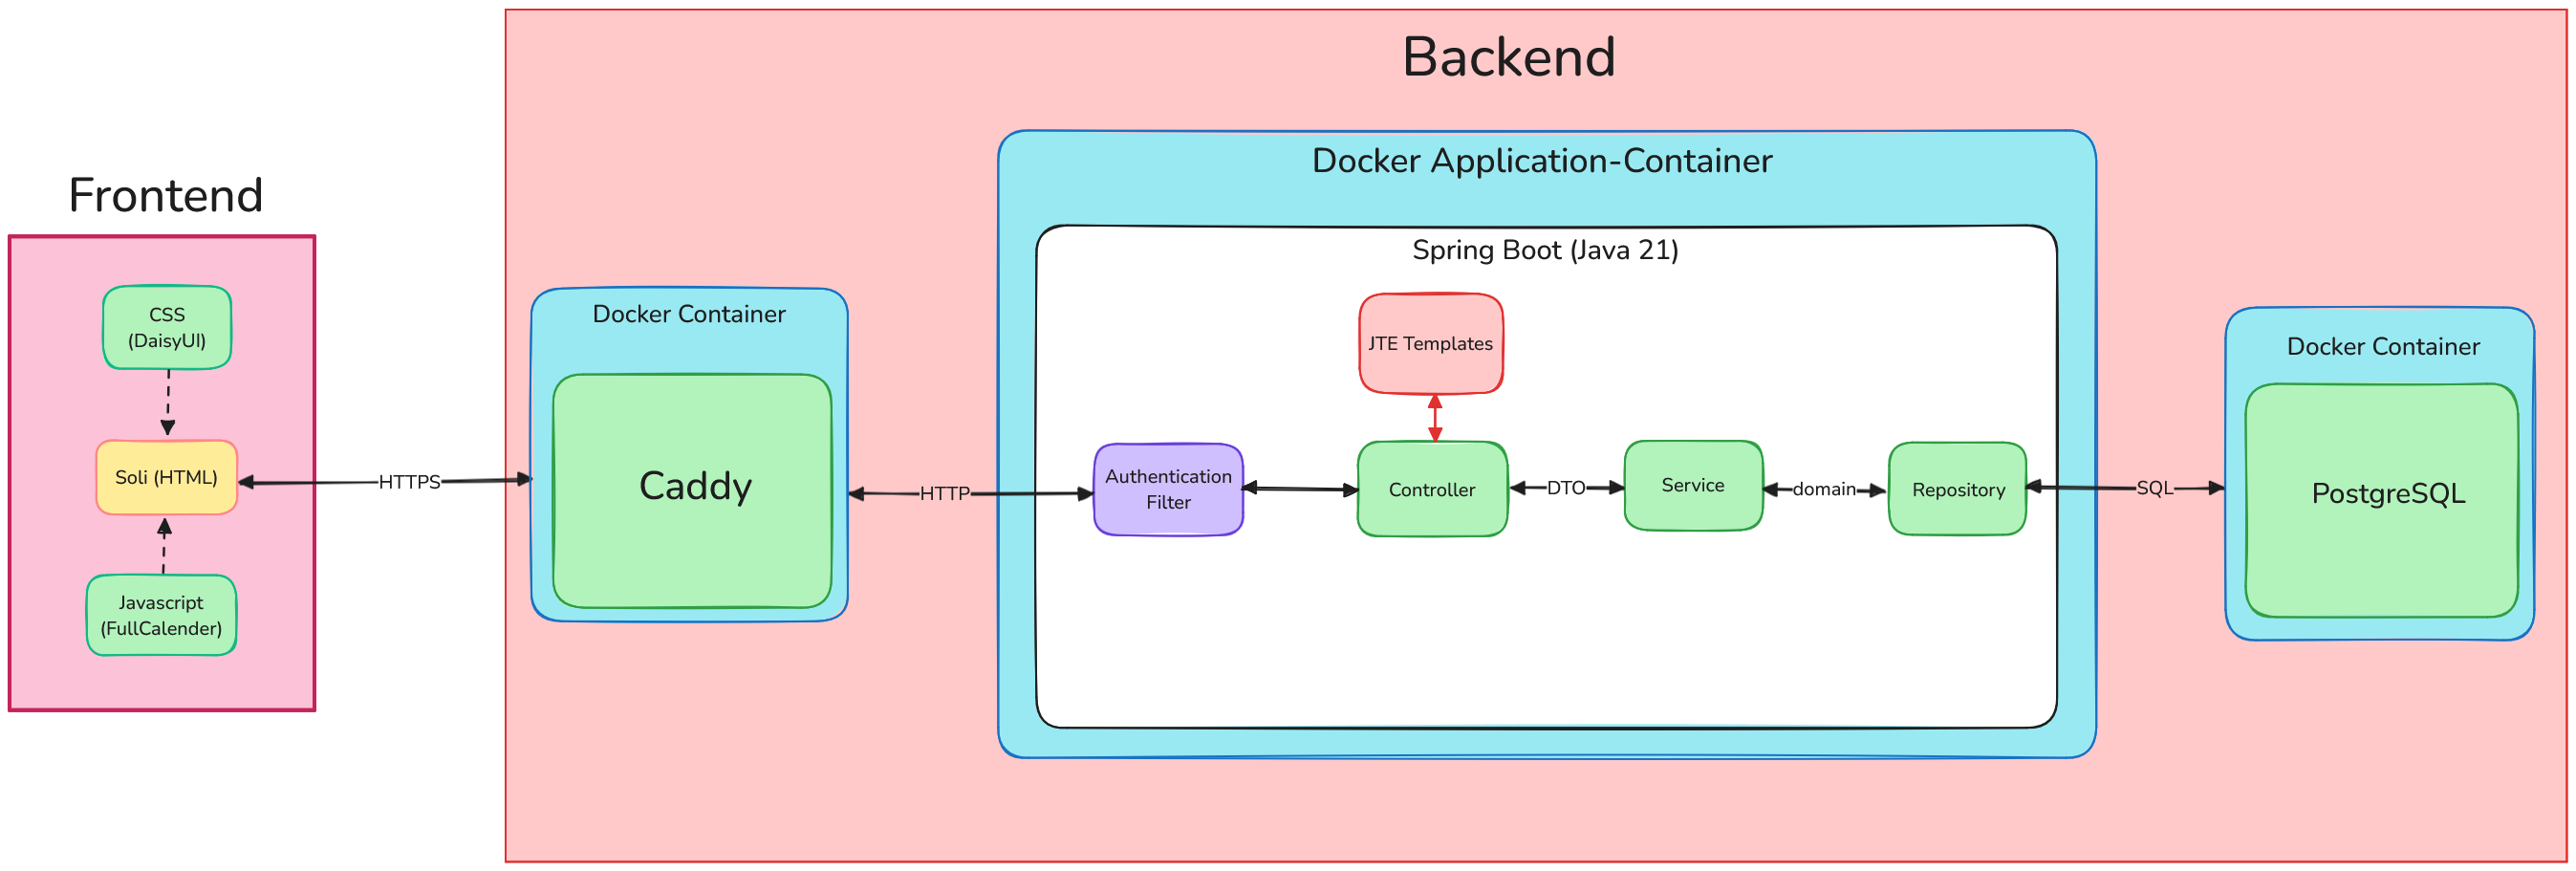
\includegraphics[width=\textwidth]{pictures/figures/architecture}
    \label{fig:architektur}
\end{figure}
\end{frame}

\subsection{Klassendiagramm}
\begin{frame}{Klassendiagramm}
    \begin{figure}
        \centering
        \includegraphics[width=\textwidth]{pictures/figures/classes}
        \caption{Bei Bedarf am Ende als einzelnes PDF danach fragen}
        \label{fig:klassendiagramm}
    \end{figure}
\end{frame}

\section{View}

\subsection{Ansichten}
\begin{frame}{Ansichten}
    \begin{itemize}
        \item \textbf{Loginansicht}: Der/die Nutzende muss die Anmeldedaten eingeben, um auf ein Großteil der Funktionalität zuzugreifen.
        \item \textbf{Kalenderansicht}: Zeigt den Kalender mit den Terminen.
        \item \textbf{Termin-Erstellen-Ansicht}: Mit ihr kann der/die Nutzende einen Termin mit Zeitraum, Priorität, und optionaler Beschreibung, sowie eine Angabe zur Bereitschaft zur geteilten Raumnutzung erstellen.
        \item \textbf{Terminansicht}: Zeigt die Informationen des Termins, sowie die Möglichkeit zur Anfrage einer geteilten Raumnutzung oder für den Eigentümer und Admin, die Möglichkeit des Termin-Löschens.
        \item \textbf{Terminübersicht}: Zeigt aufgelistet alle gebuchten Termine des Nutzenden, sowie die Möglichkeit Termine zu löschen und anzusehen.
        \item \textbf{Kontenliste}: Nur für Admins zugänglich und bietet die Möglichkeit spezifische Nutzende zu verbannen oder die Gästefunktionalität auszuschalten.
    \end{itemize}
\end{frame}

\subsection{Anmeldungsansicht}
\begin{frame}{Anmeldungsansicht}
    \begin{figure}
        \centering
        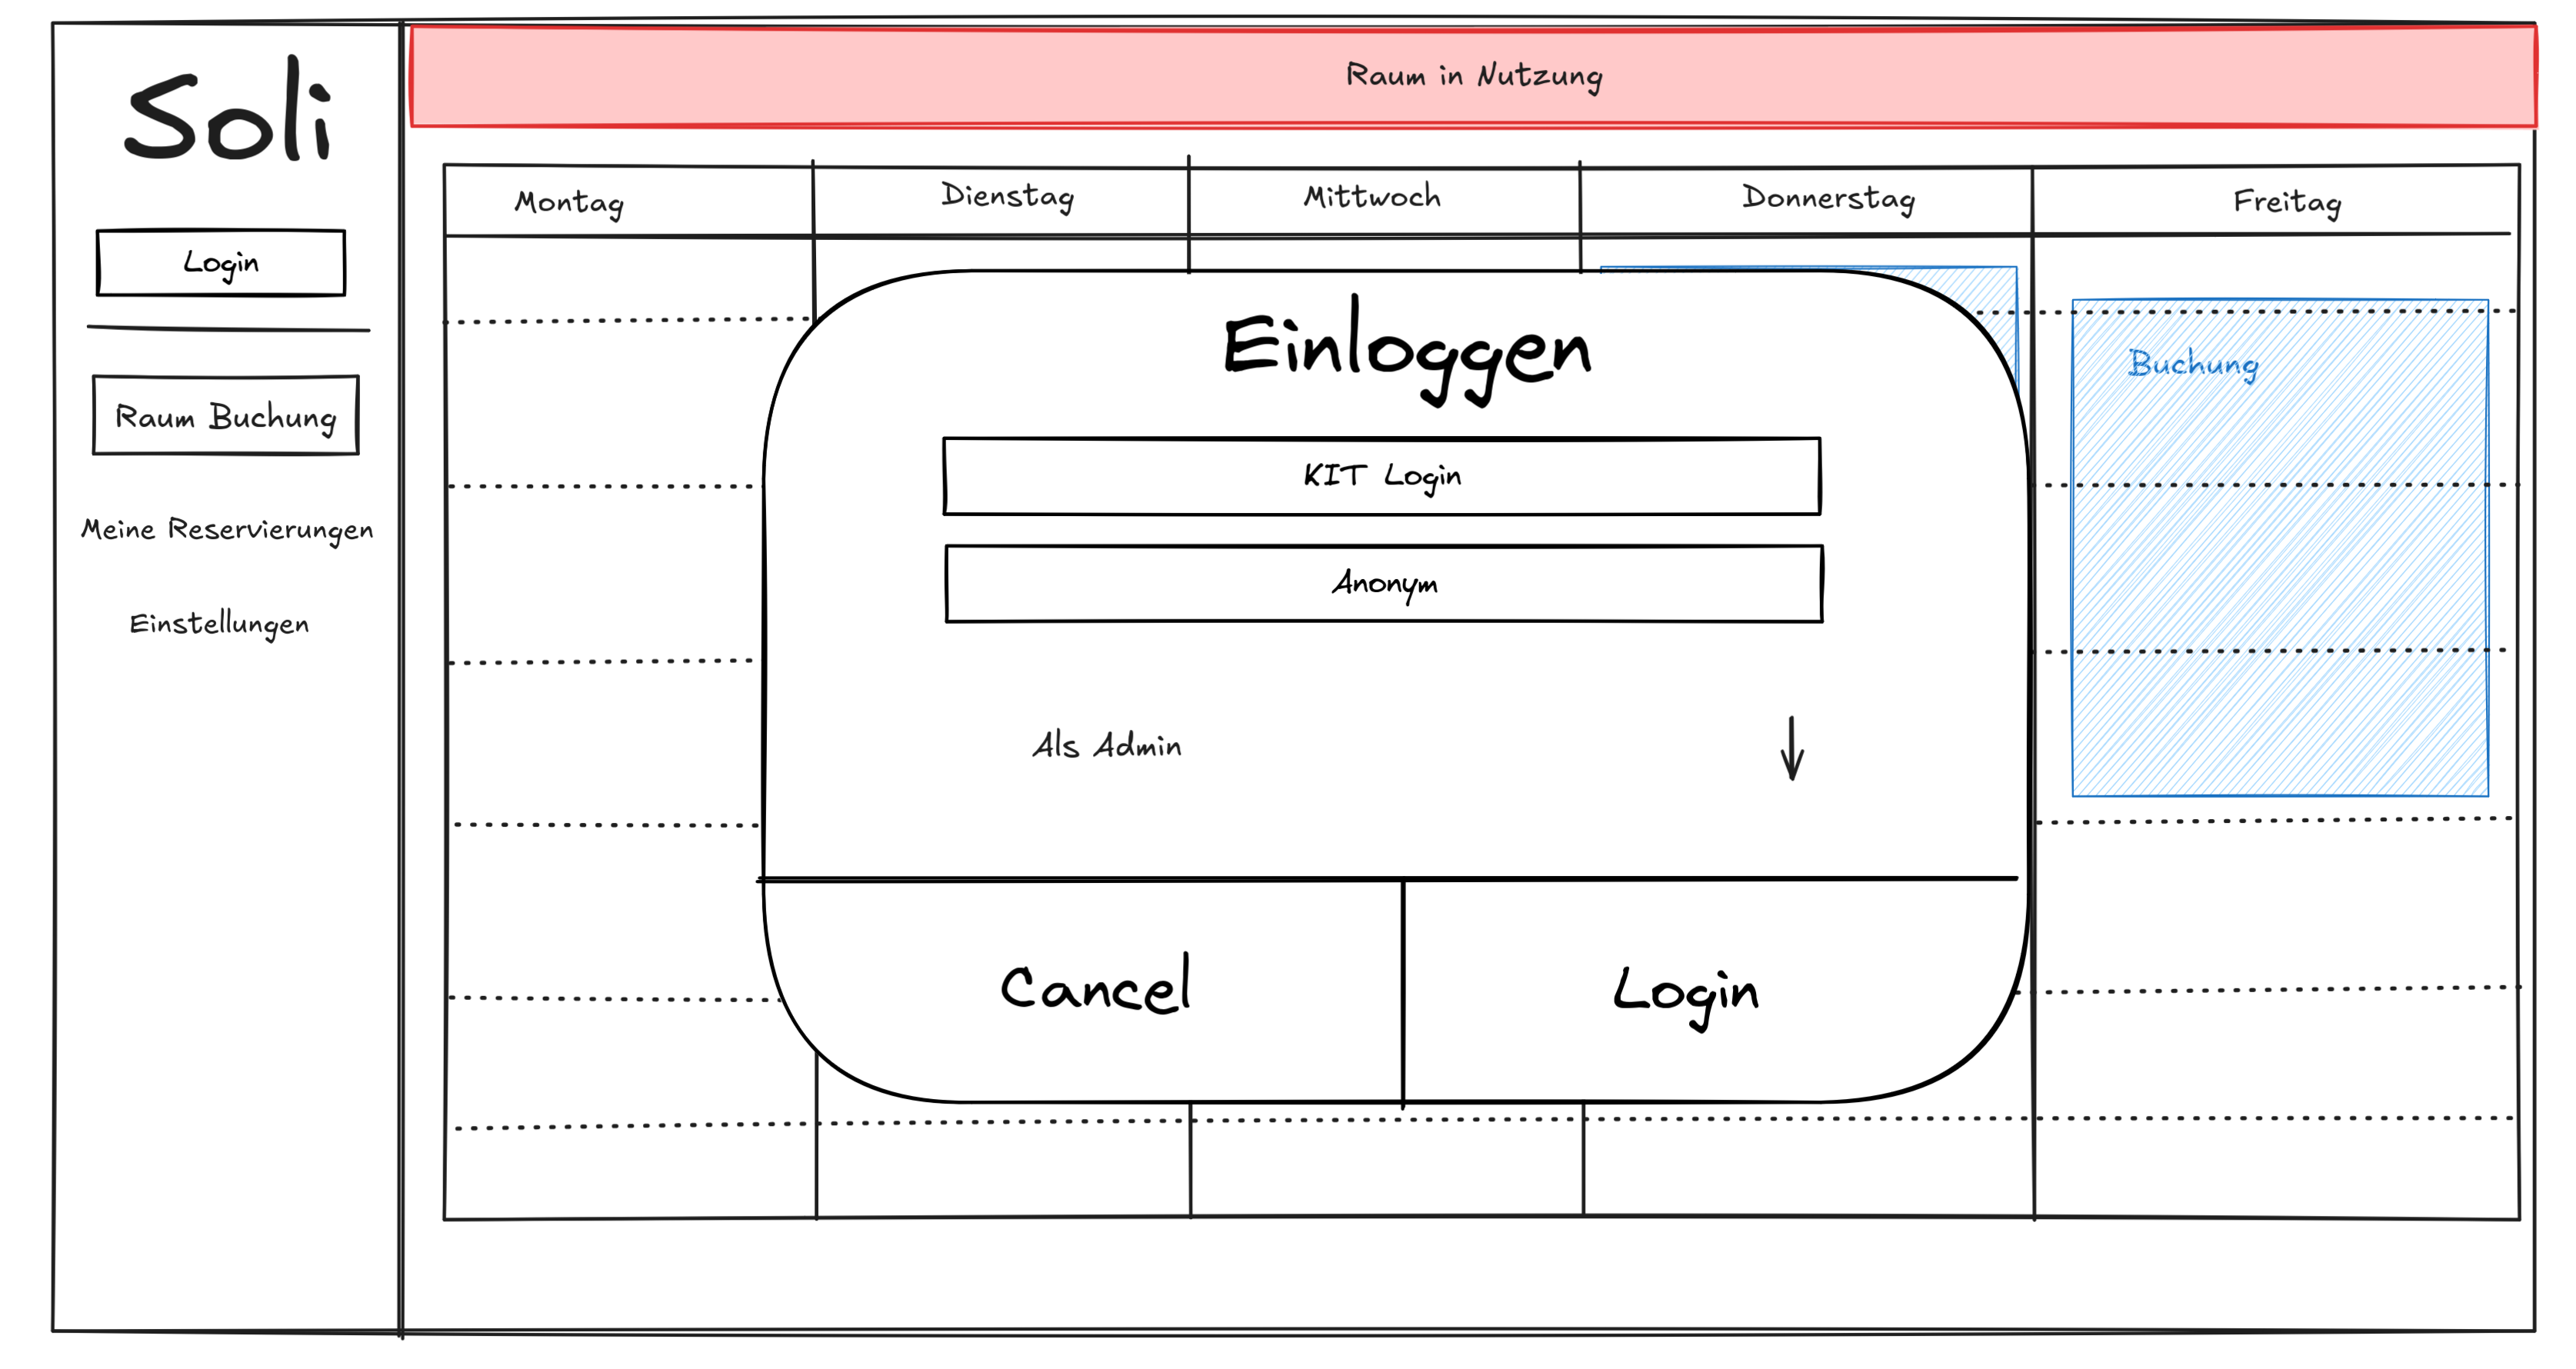
\includegraphics[width=\textwidth]{pictures/figures/ui/anmeldungsseite}
        \label{fig:login}
    \end{figure}
\end{frame}

\begin{frame}
    \begin{figure}
        \centering
        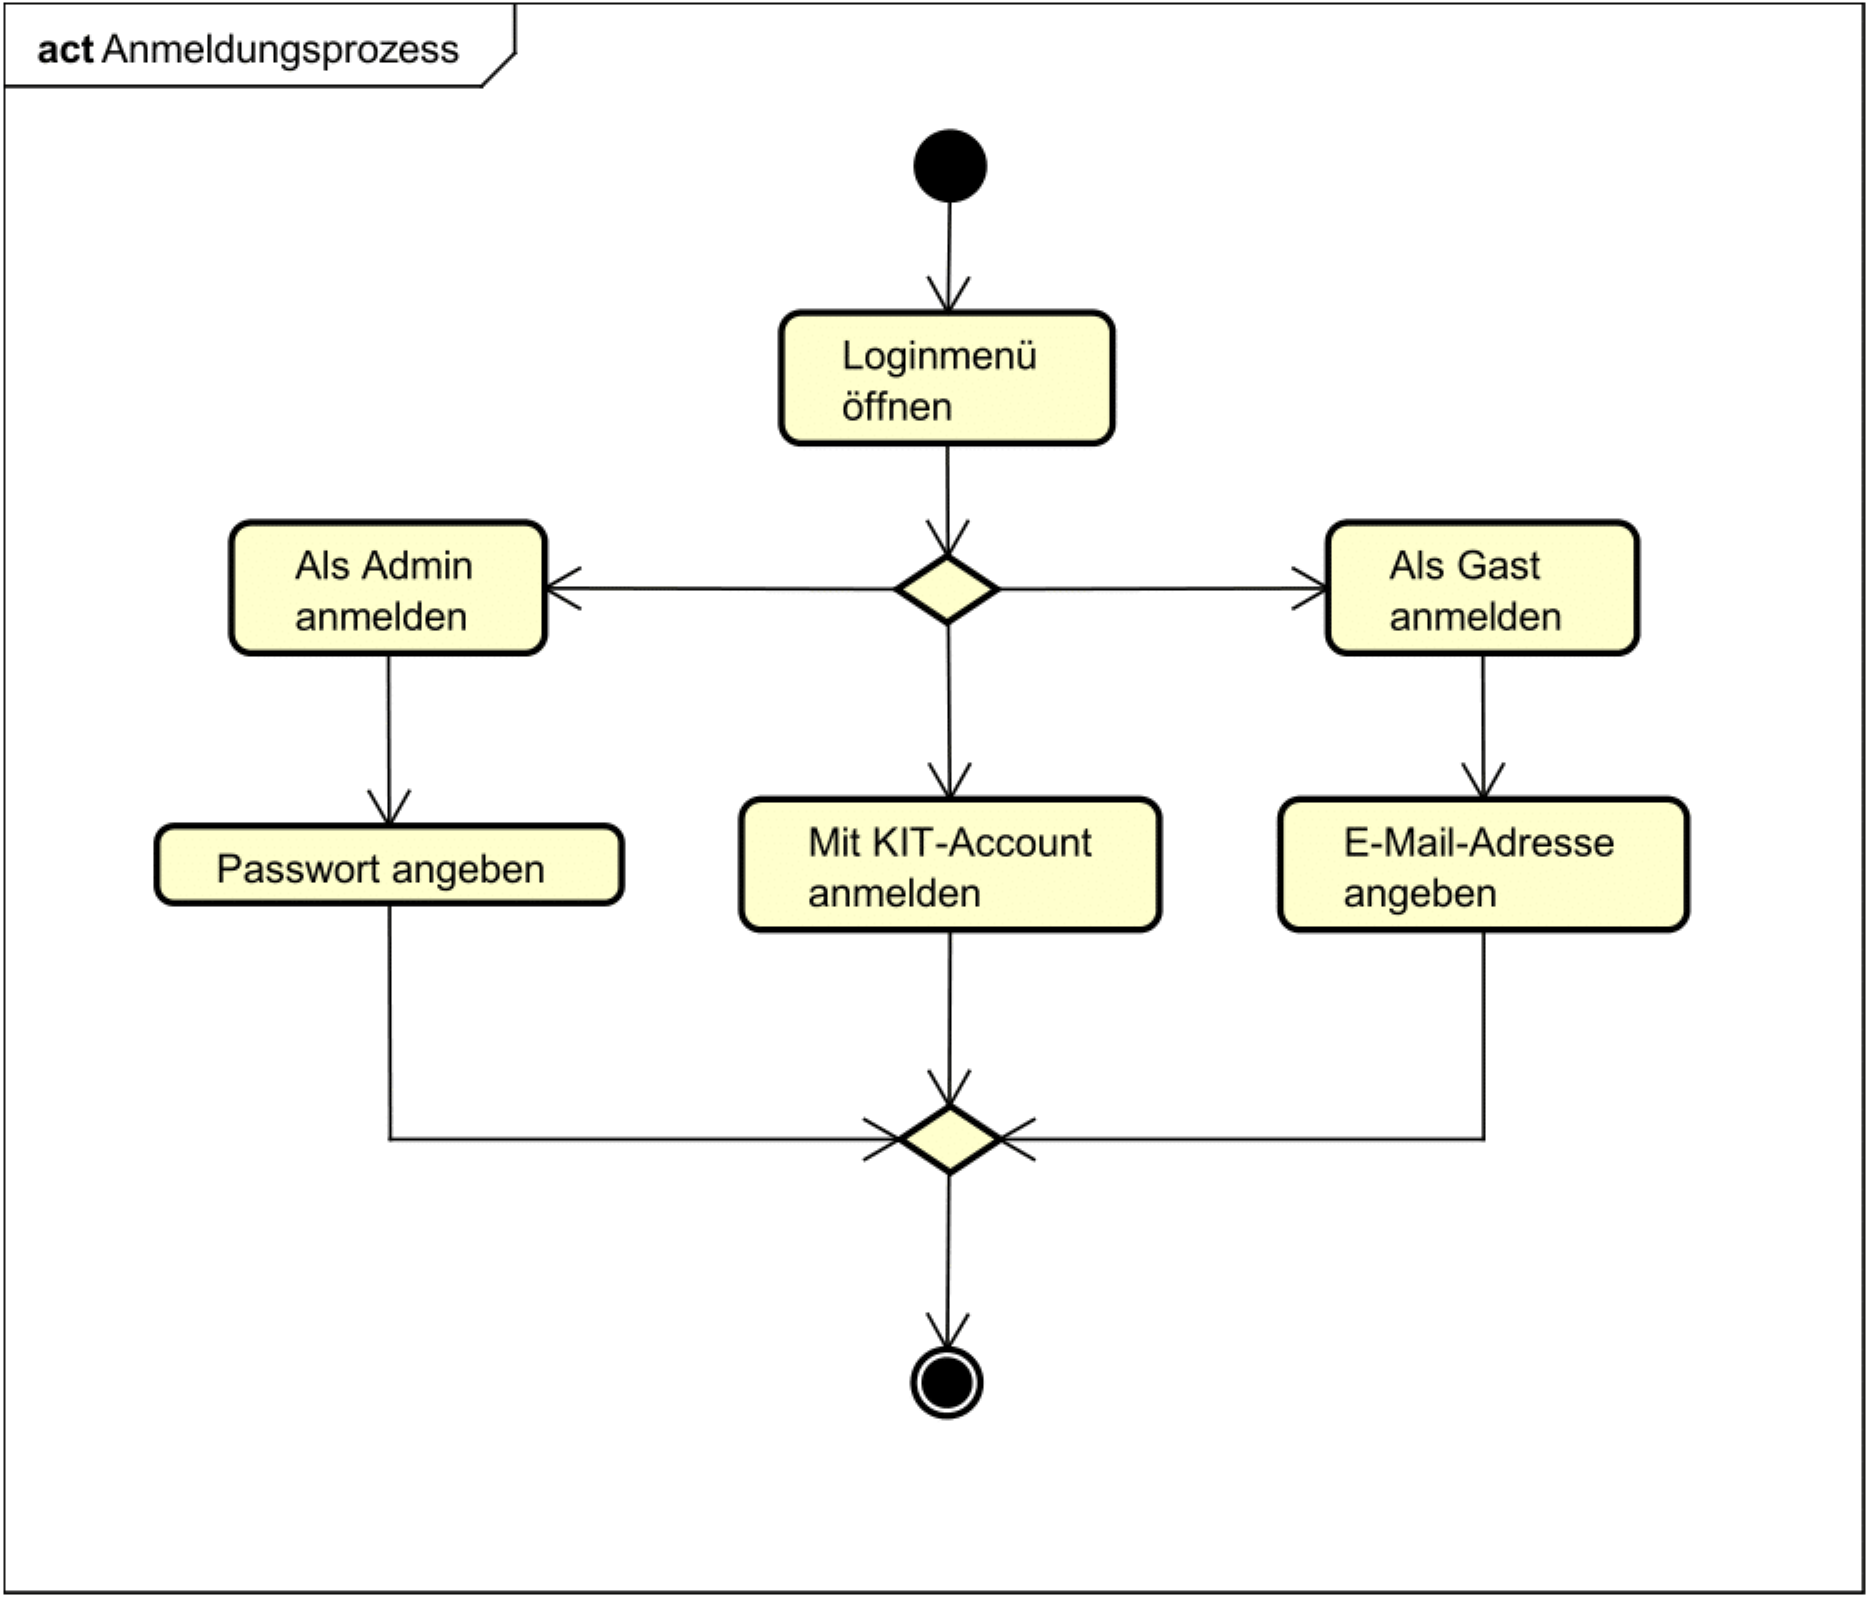
\includegraphics[width=\textwidth]{pictures/figures/activity/anmeldeprozess}
        \caption{Mit der Anmeldung akzeptiert nun der Authentication Filter und der Großteil der Funktionalität ist nun zugänglich.}
        \label{fig:loginprozess}
    \end{figure}
\end{frame}

\subsection{Kalenderansicht}
\begin{frame}{Kalenderansicht}
    \begin{figure}
        \centering
        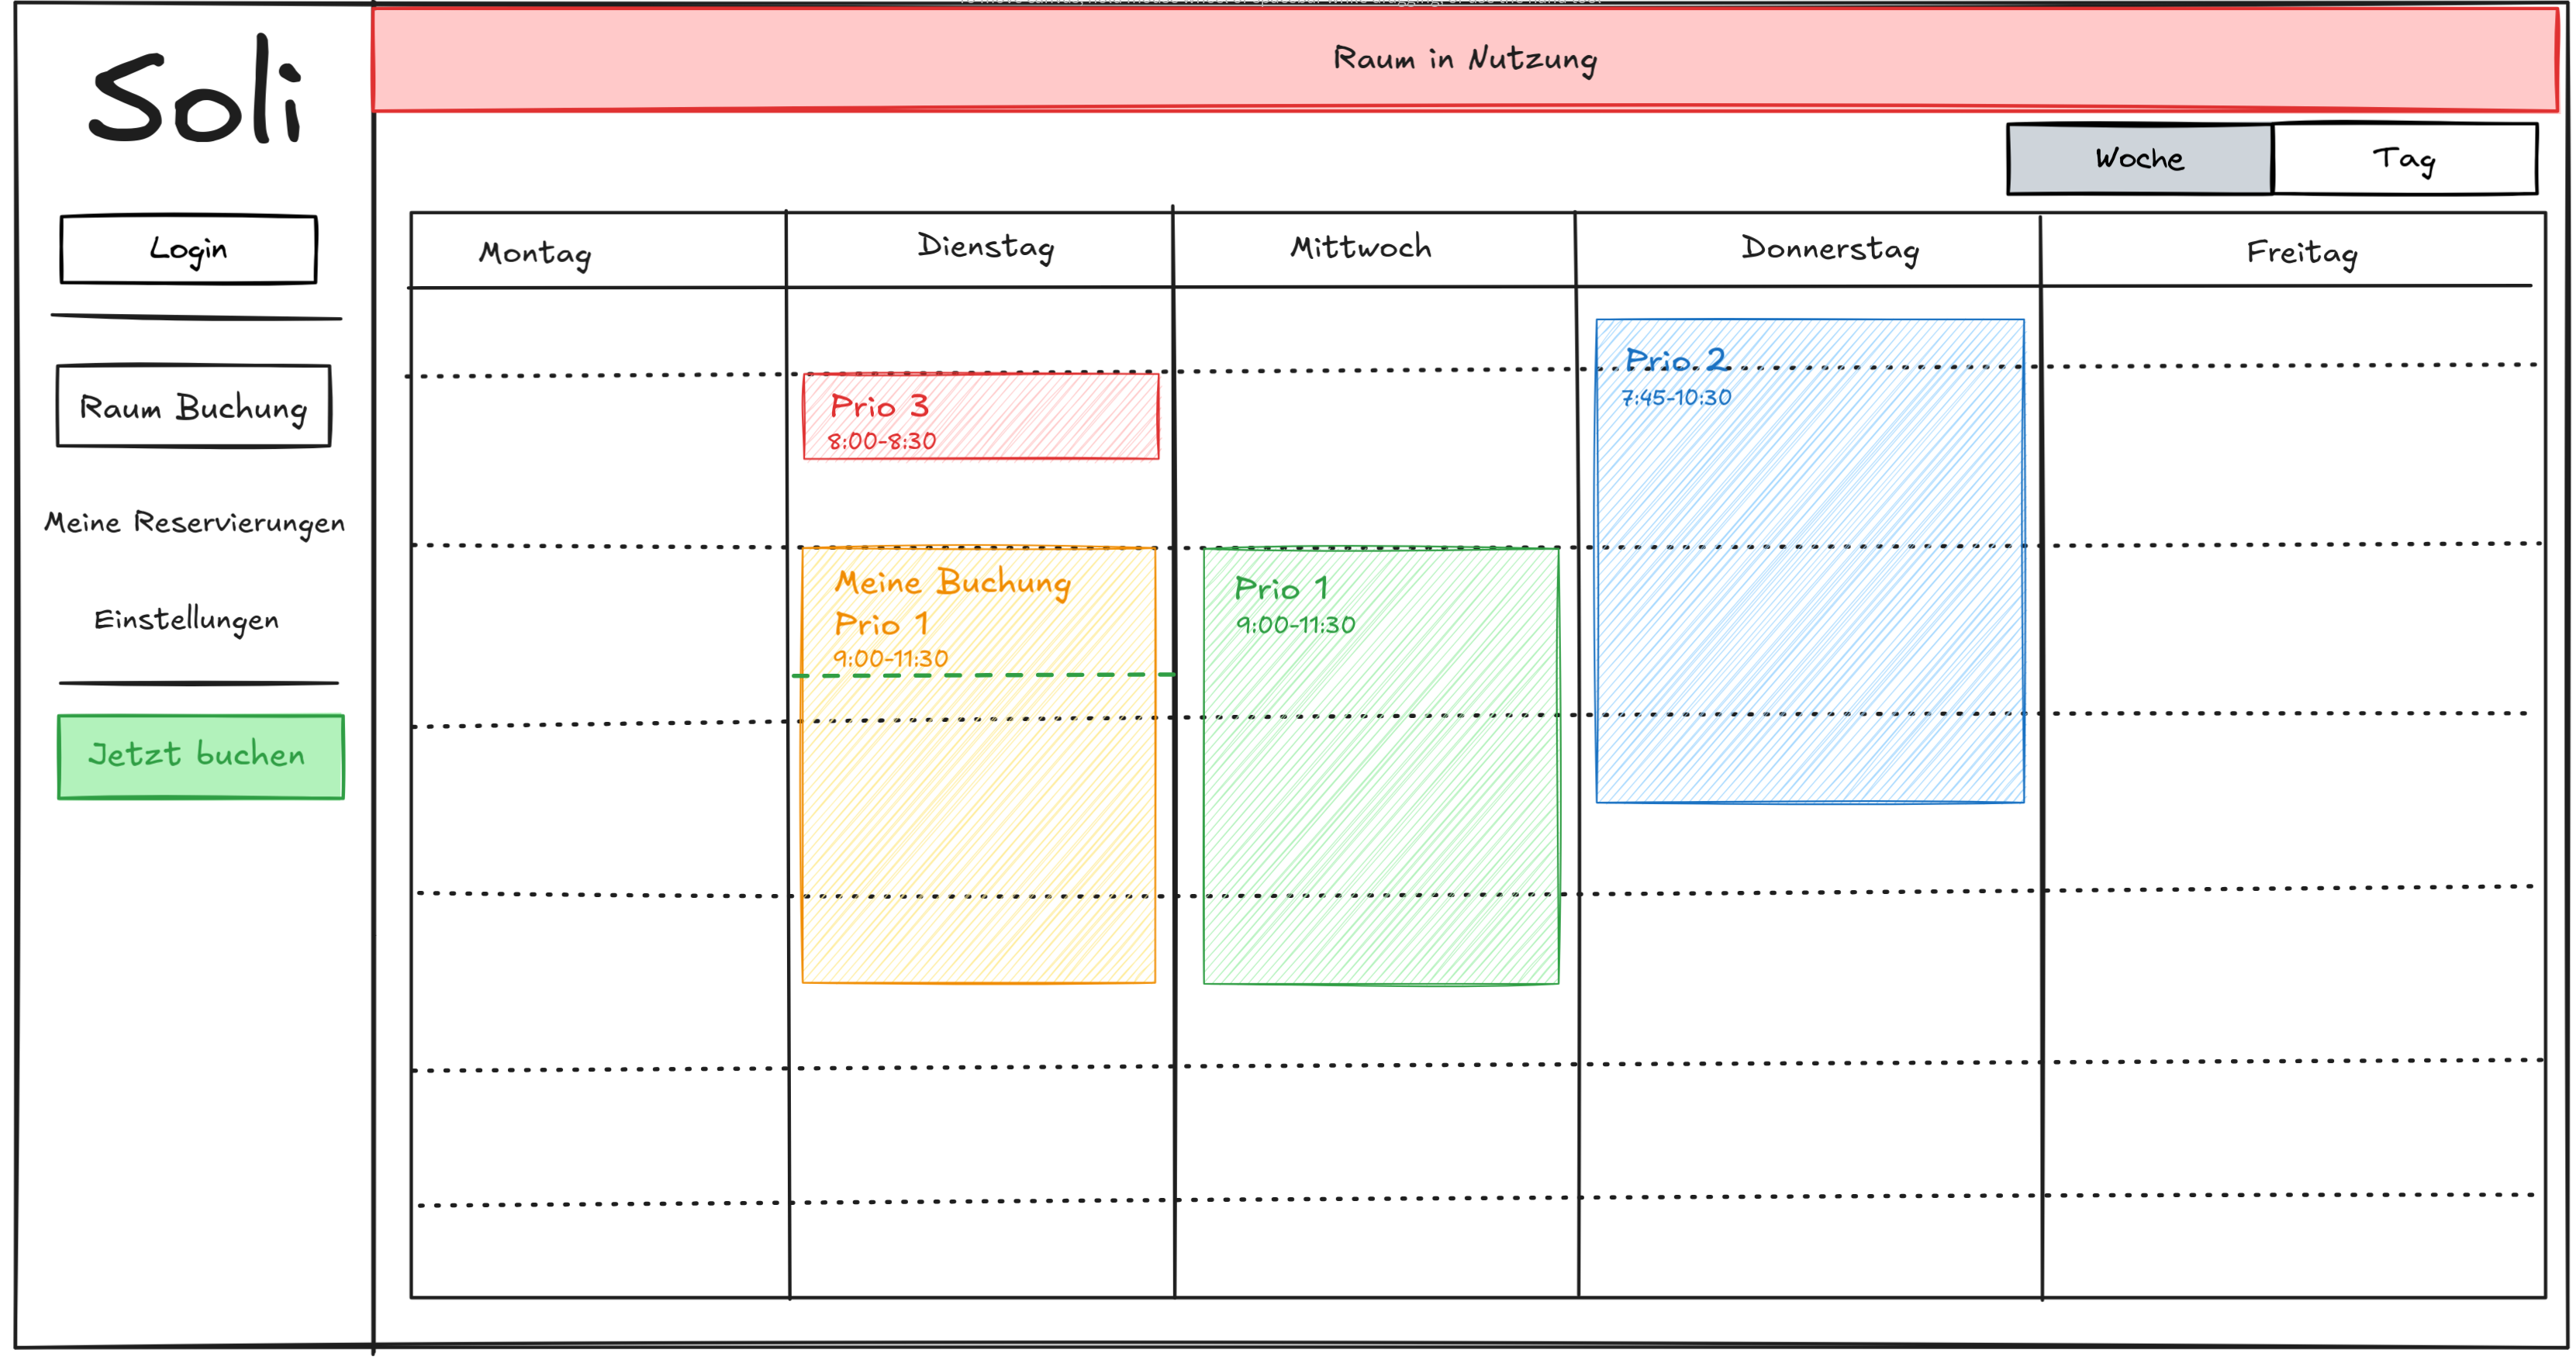
\includegraphics[width=\textwidth]{pictures/figures/ui/startseite}
        \caption{Zeigt alle Termine an, die in der Datenbank gespeichert sind.}
        \label{fig:kalender}
    \end{figure}
\end{frame}

\subsection{Termin-Erstellen-Ansicht}
\begin{frame}
    \begin{figure}
        \centering
        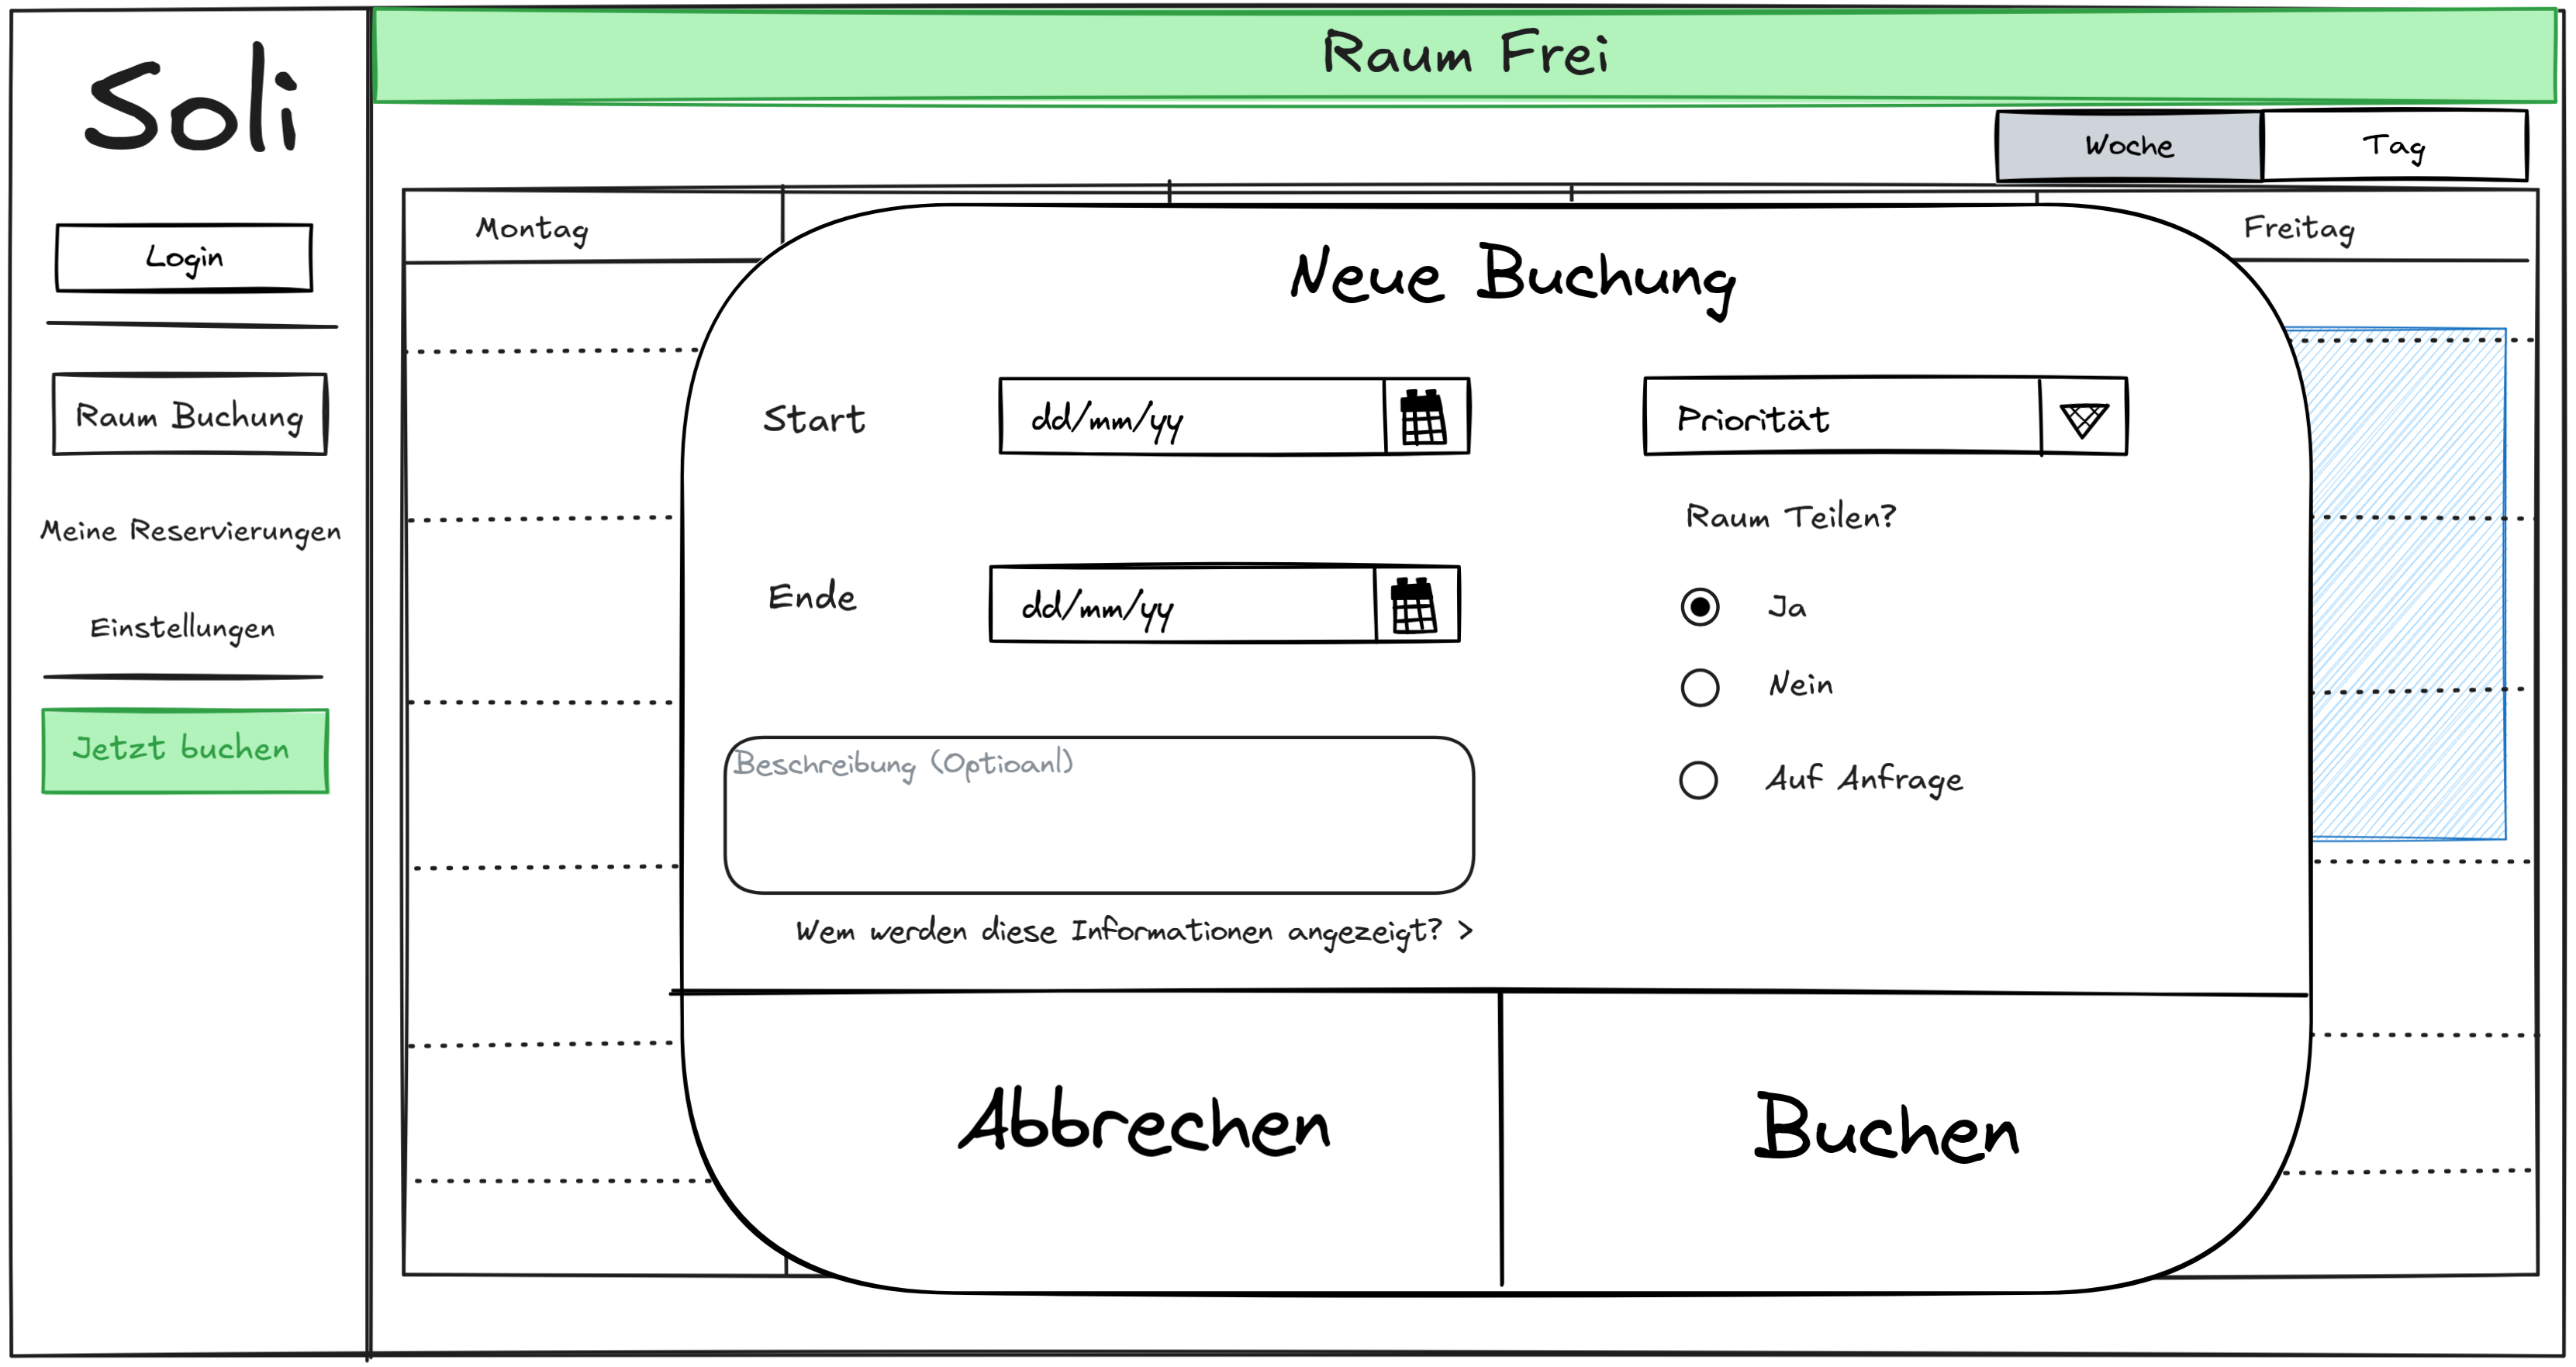
\includegraphics[width=\textwidth]{pictures/figures/ui/buchungsdialog}
        \caption{Diese Ansicht wird über die Kalenderansicht erreicht.}
        \label{fig:terminerstellen}
    \end{figure}
\end{frame}

\begin{frame}
    \begin{figure}
        \centering
        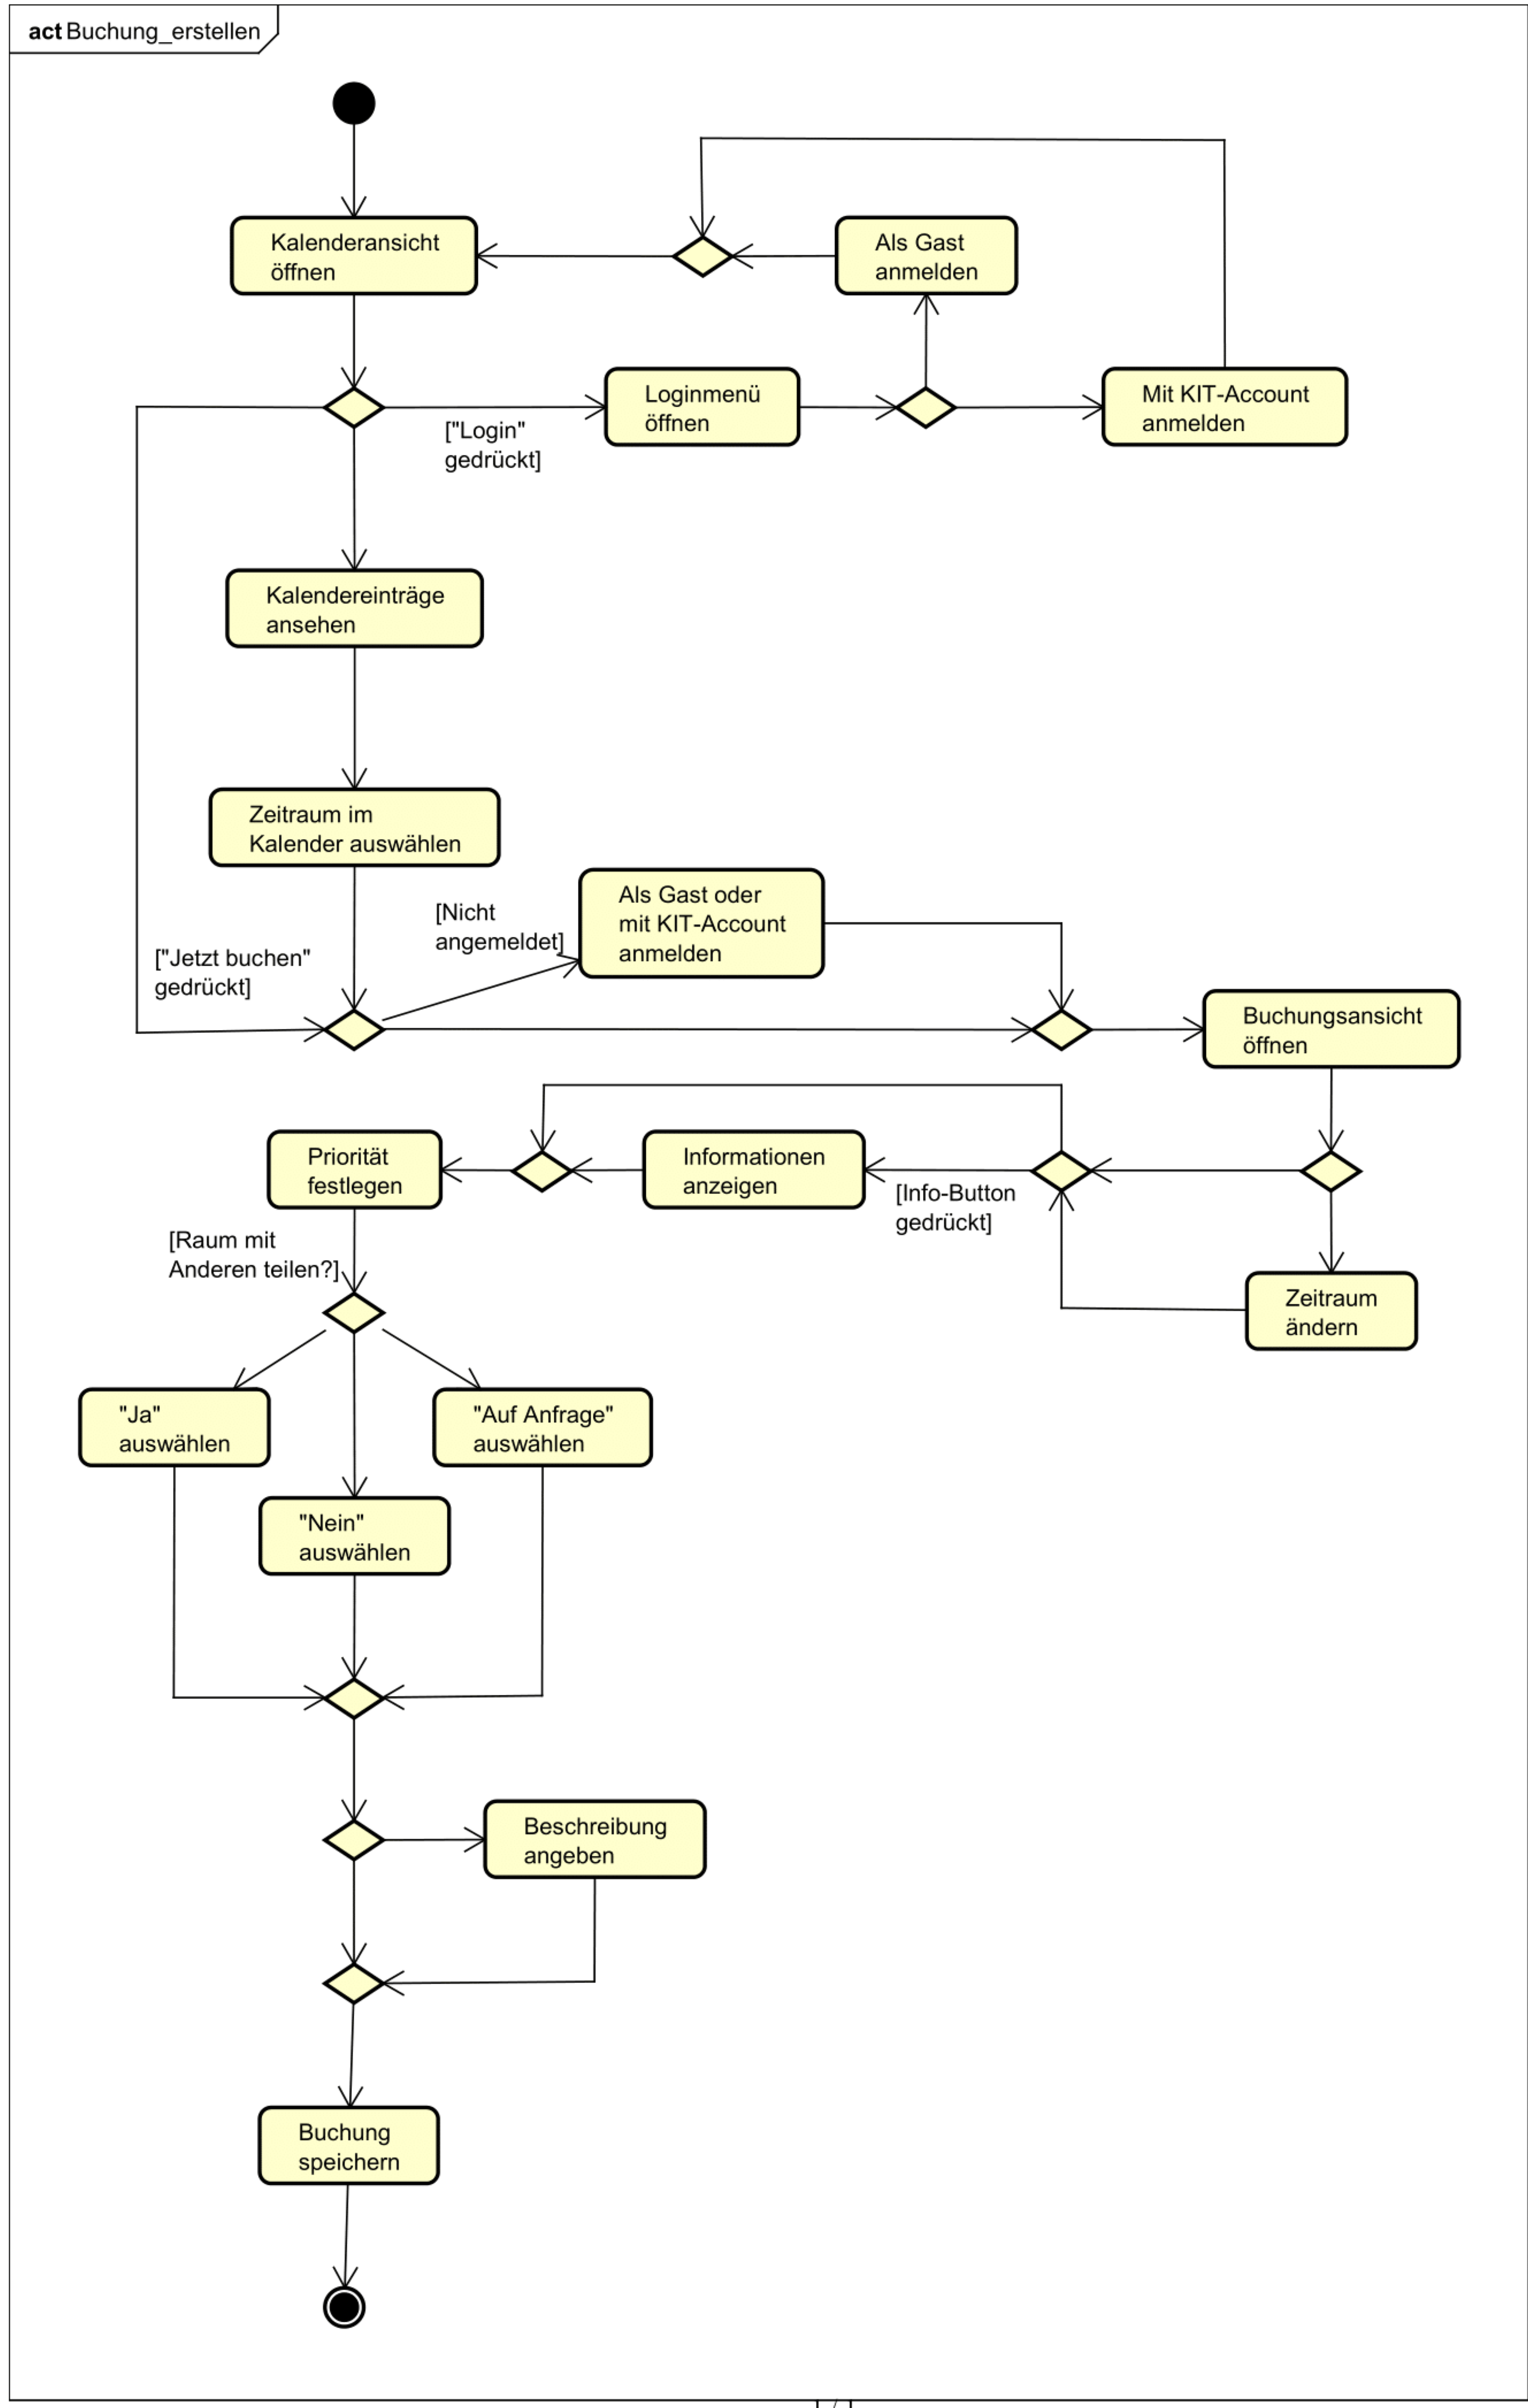
\includegraphics[width=\textwidth]{pictures/figures/activity/buchungerstellen} % TODO Bild in 2 Teile splitten
        \caption{Der Termin wird in der Datenbank gespeichert und ist nun in der Kalenderansicht sichtbar.}
        \label{fig:terminerstellenprozess}
    \end{figure}
\end{frame}

% TODO Frame für Sequenzdiagramm Terminerstellen
% TODO Frame für Erklärung des Terminerstellenprozesses

\subsubsection{Terminkonfliktlösung}
\begin{frame}{Terminkonfliktlösung}
    \begin{figure}
        \centering
        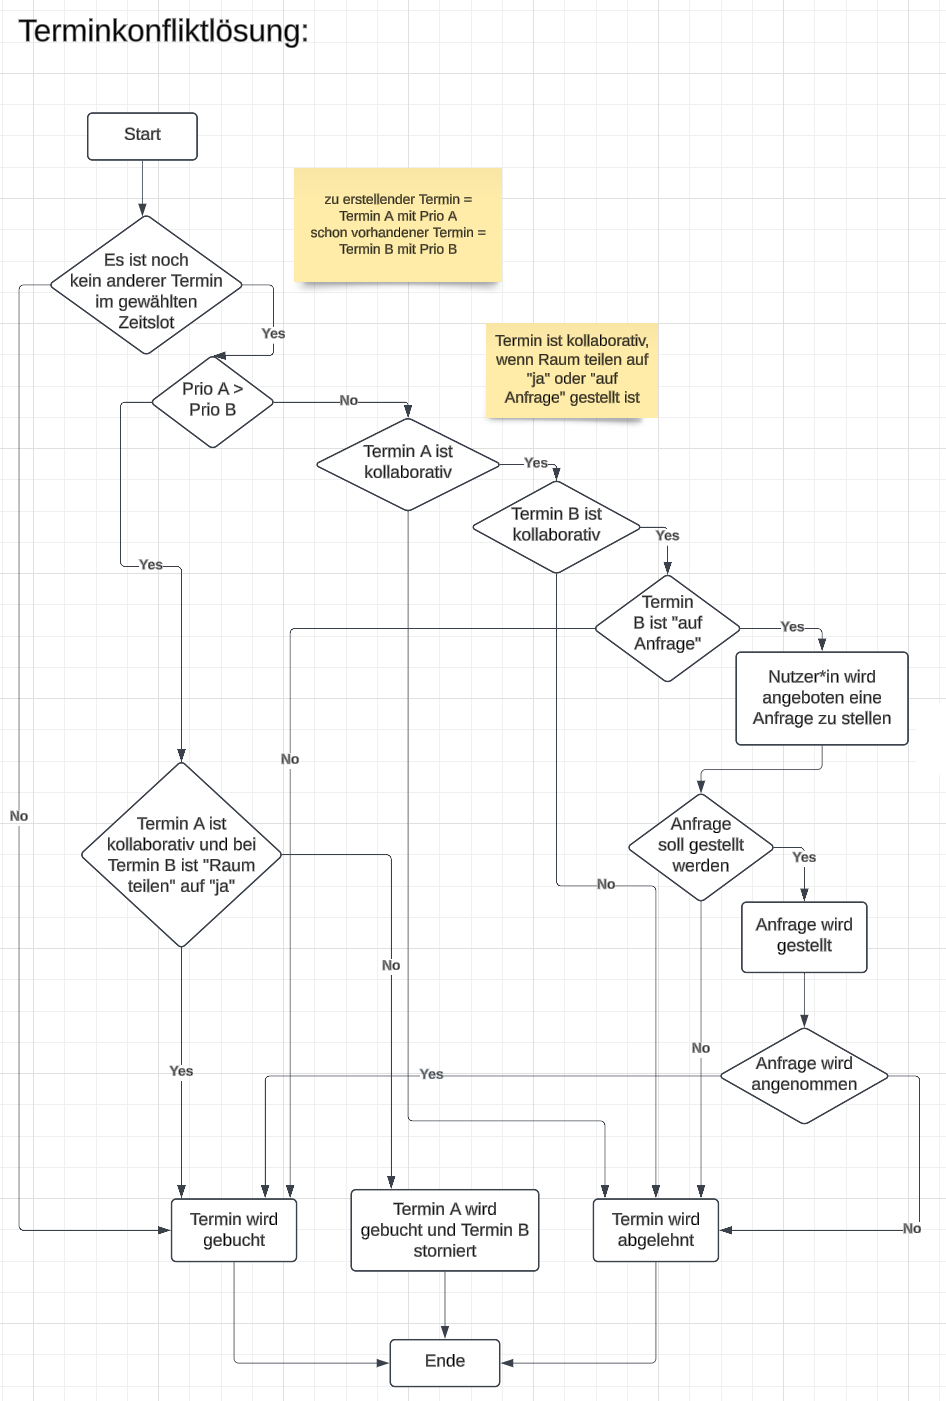
\includegraphics[width=\textwidth]{pictures/figures/activity/terminkonfliktloesung} % TODO Bild anpassen
        \label{fig:terminkonflikt}
    \end{figure}
\end{frame}

\subsection{Terminübersicht}
\begin{frame}{Terminübersicht}
    \begin{figure}
        \centering
        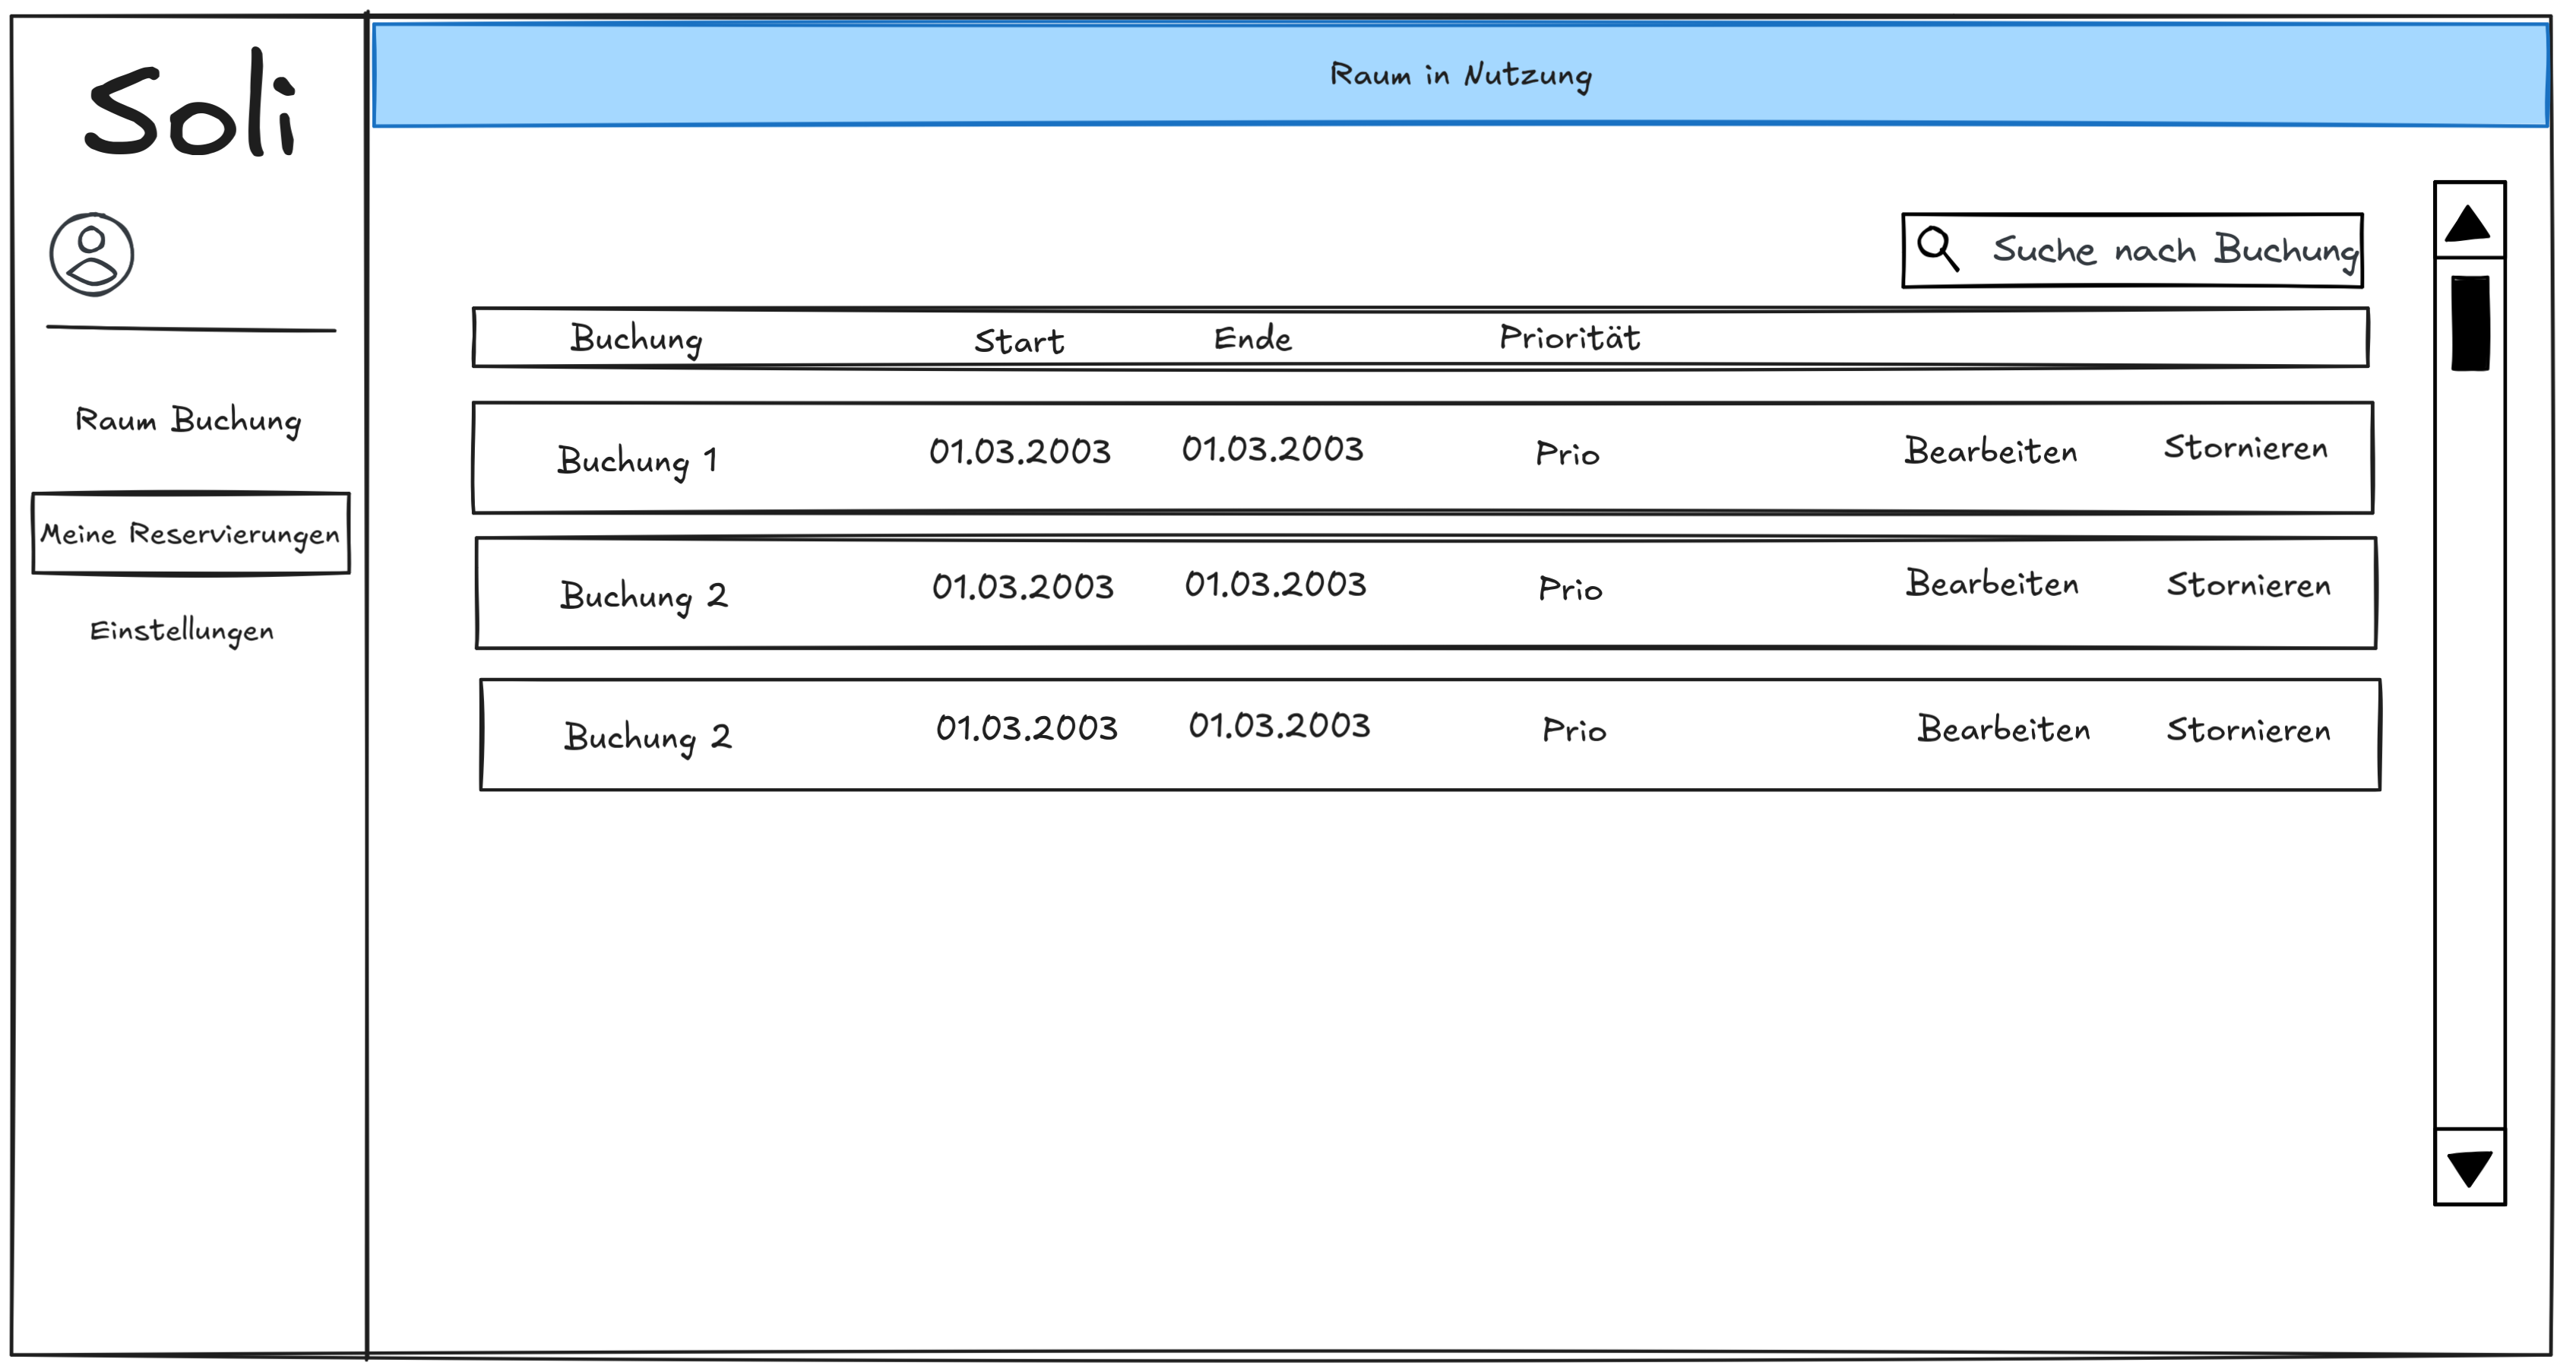
\includegraphics[width=\textwidth]{pictures/figures/ui/reservierungsuebersicht}
        \caption{Zeigt alle Termine an, die der/die Nutzende erstellt hat.}
        \label{fig:terminuebersicht}
    \end{figure}
\end{frame}

\begin{frame}
    \begin{figure}
        \centering
        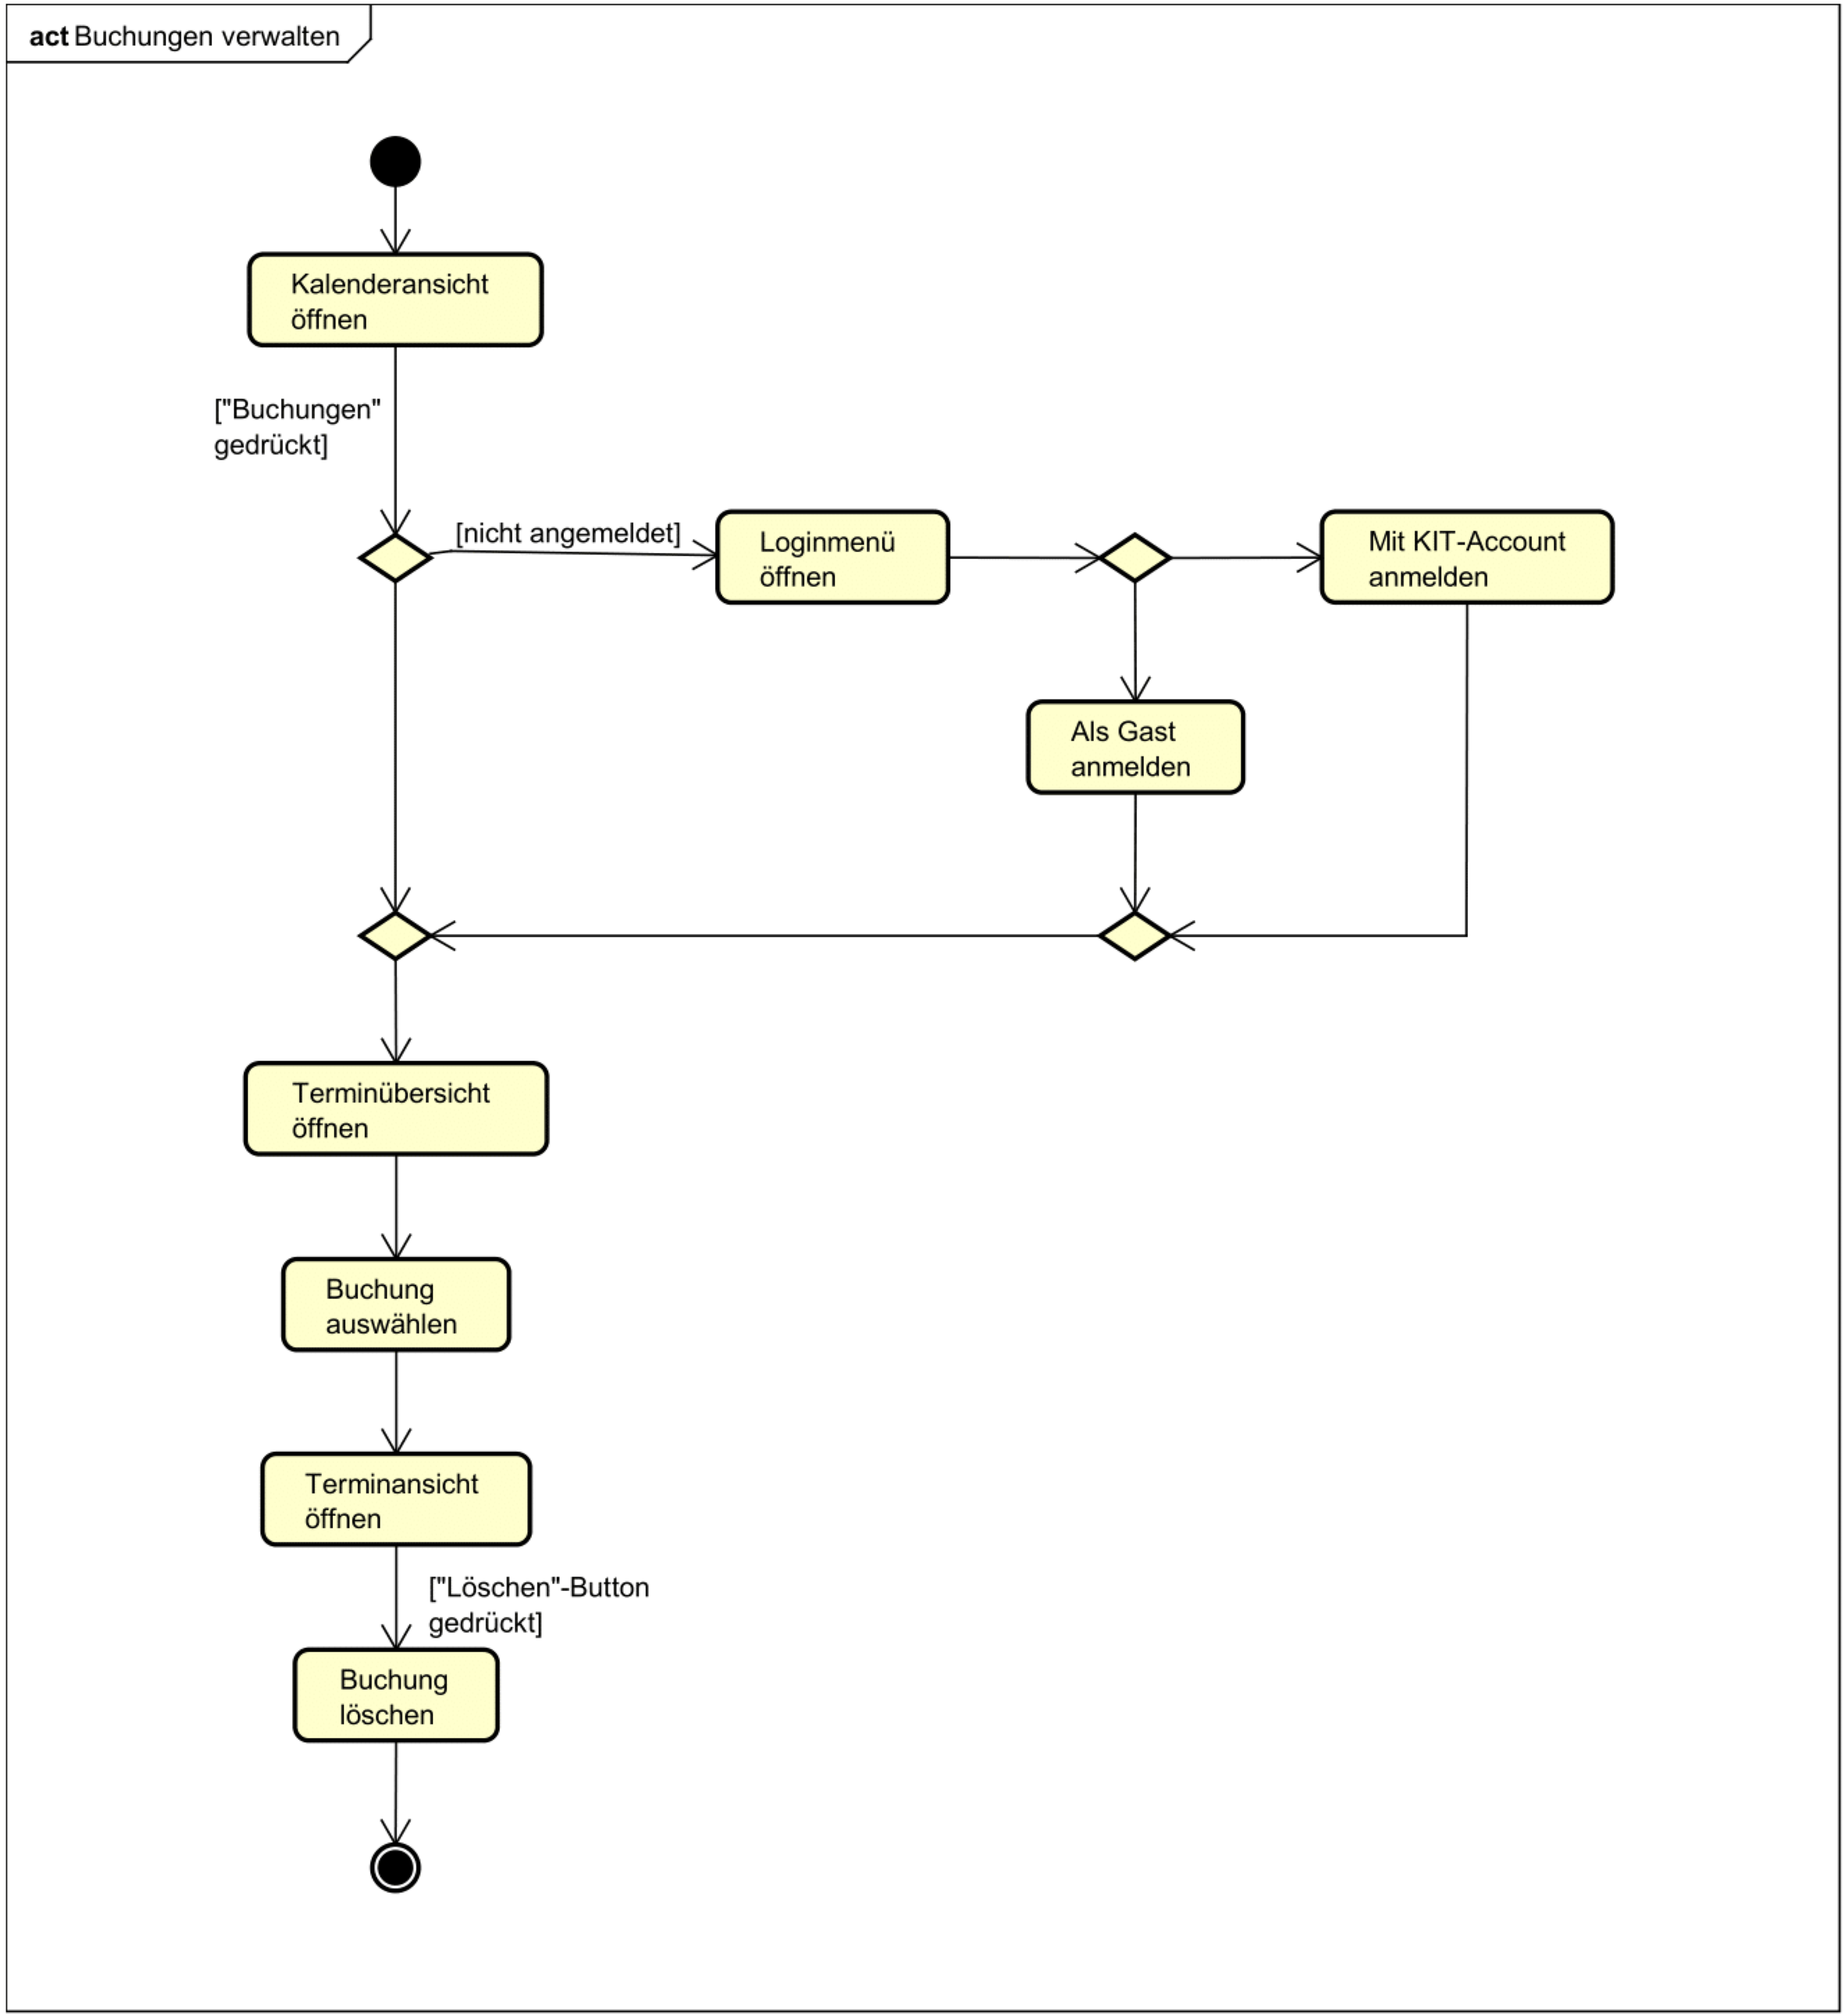
\includegraphics[width=\textwidth]{pictures/figures/activity/buchungverwalten}
        \label{fig:terminuebersichtprozess}
    \end{figure}
\end{frame}

\subsection{Terminansicht}
\begin{frame}{Terminansicht}
    \begin{figure}
        \centering
        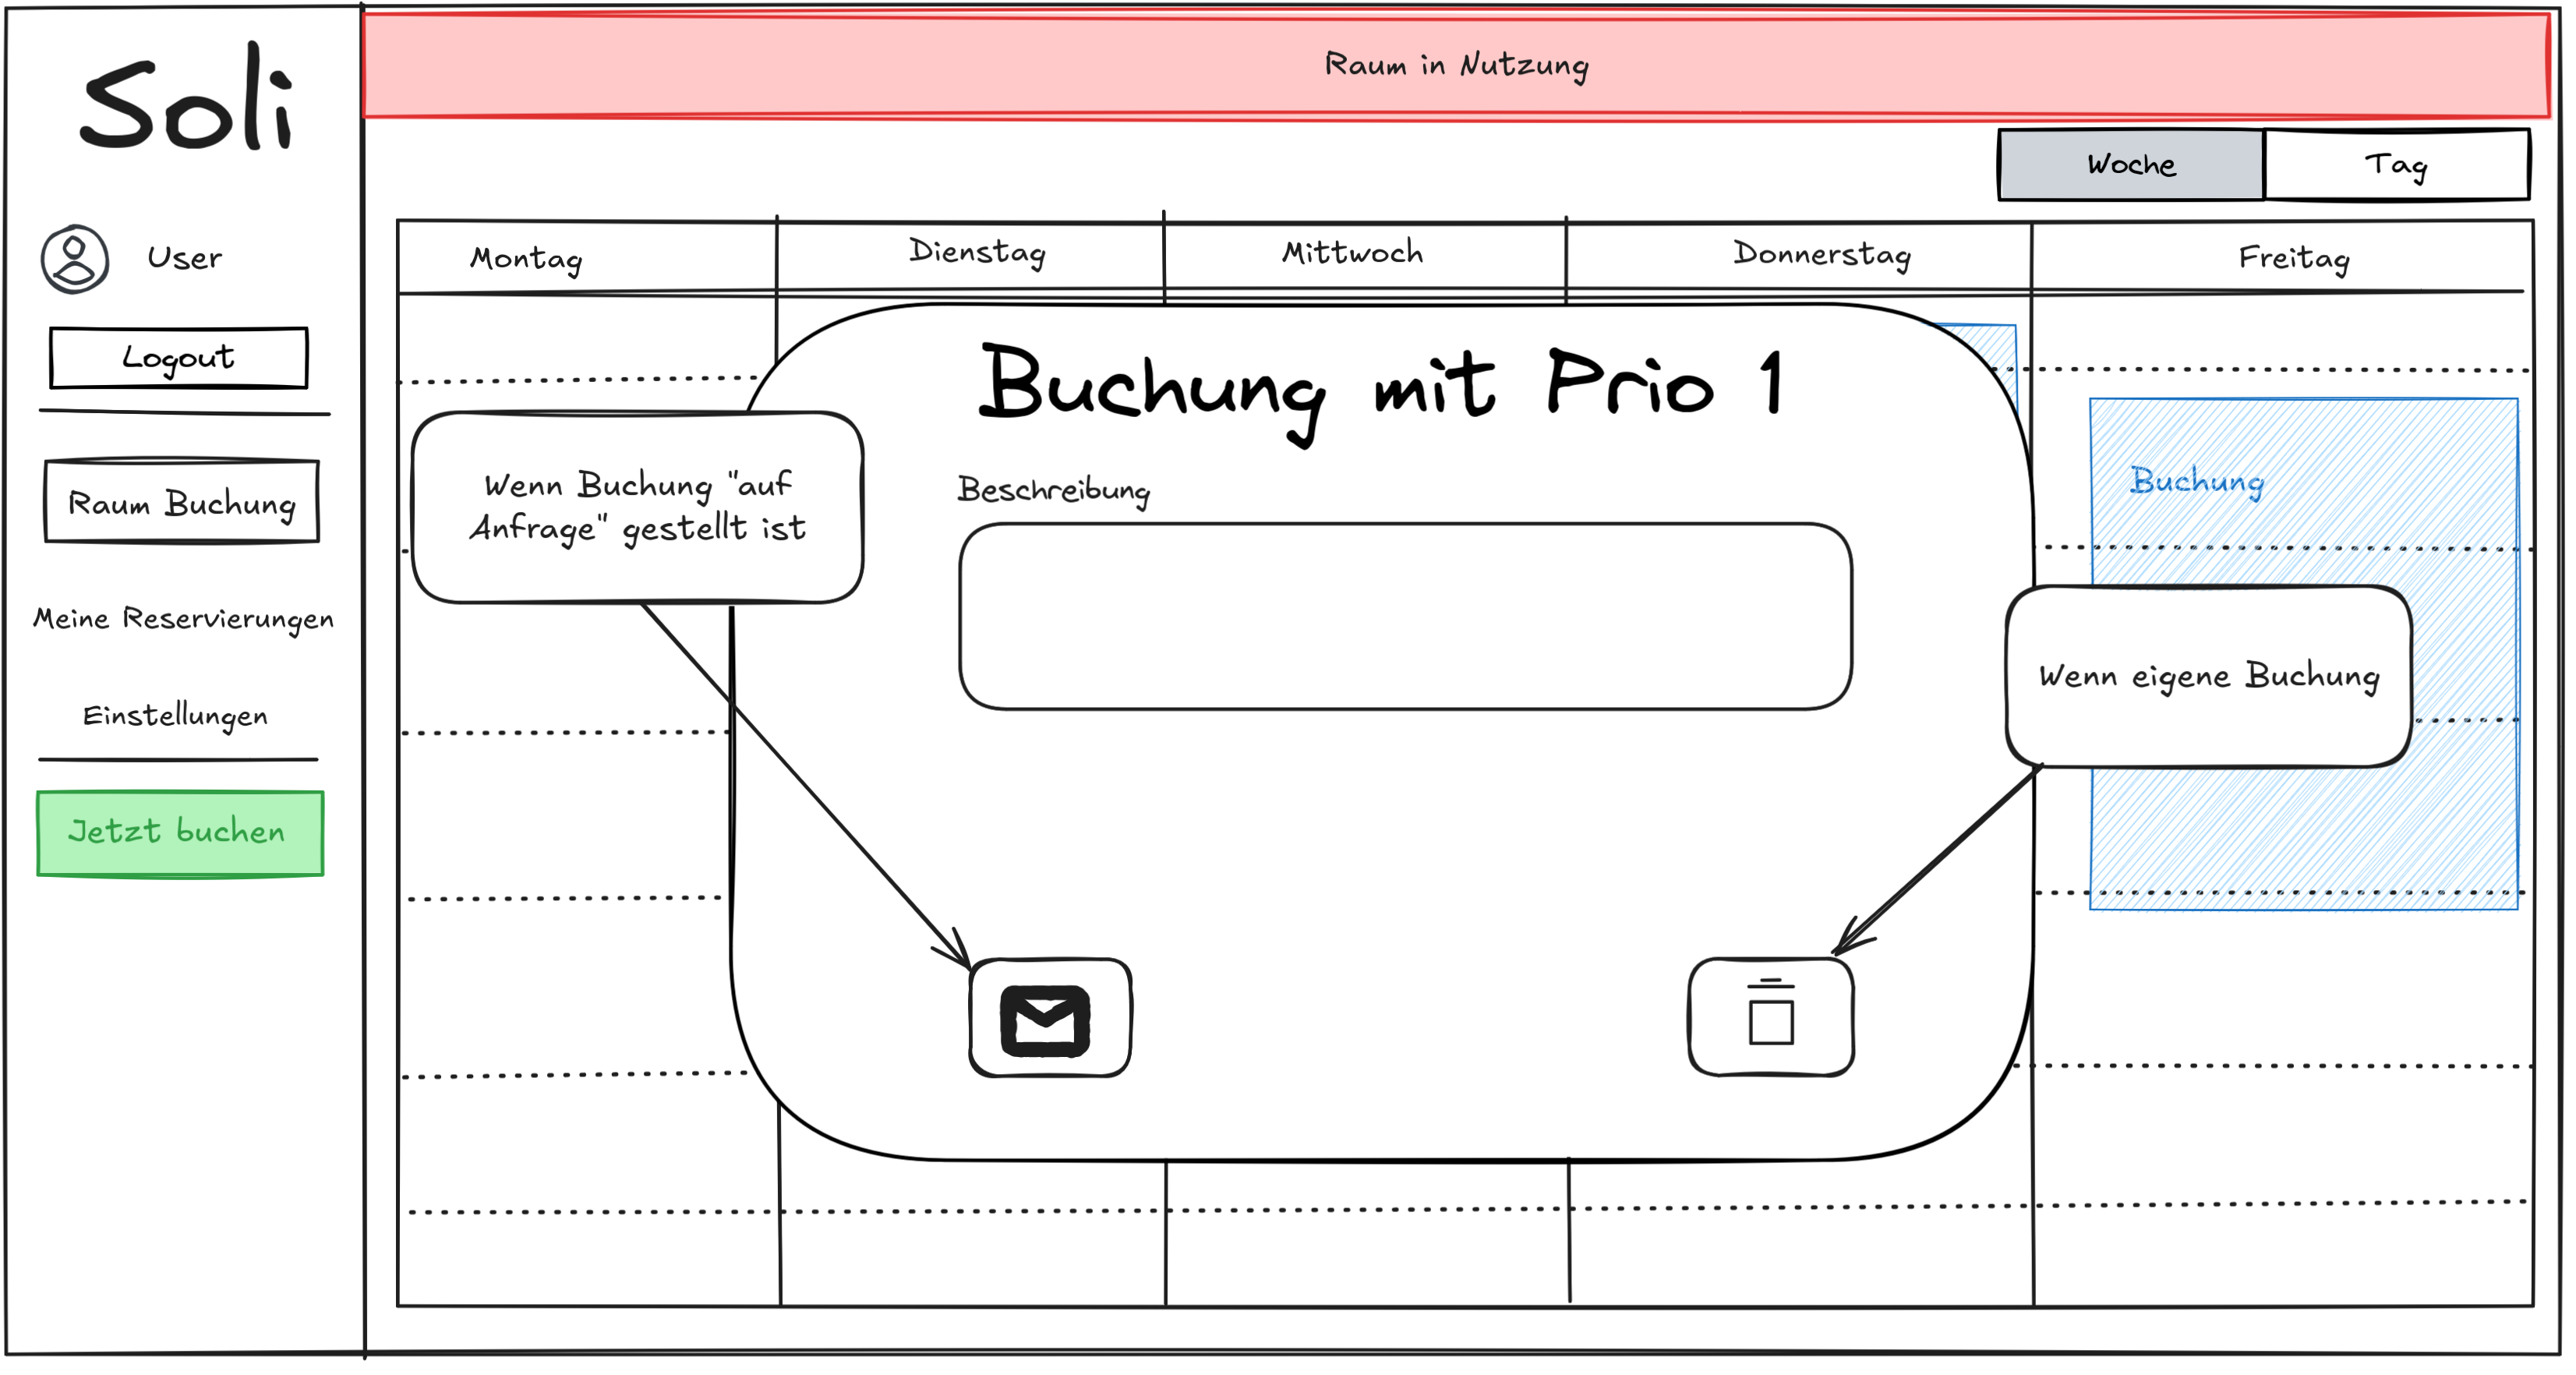
\includegraphics[width=\textwidth]{pictures/figures/ui/reservierunginkalendar}
        \caption{Zeigt alle Informationen des Termins an.}
        \label{fig:terminansicht}
    \end{figure}
\end{frame}

\begin{frame}
    \begin{figure}
        \centering
        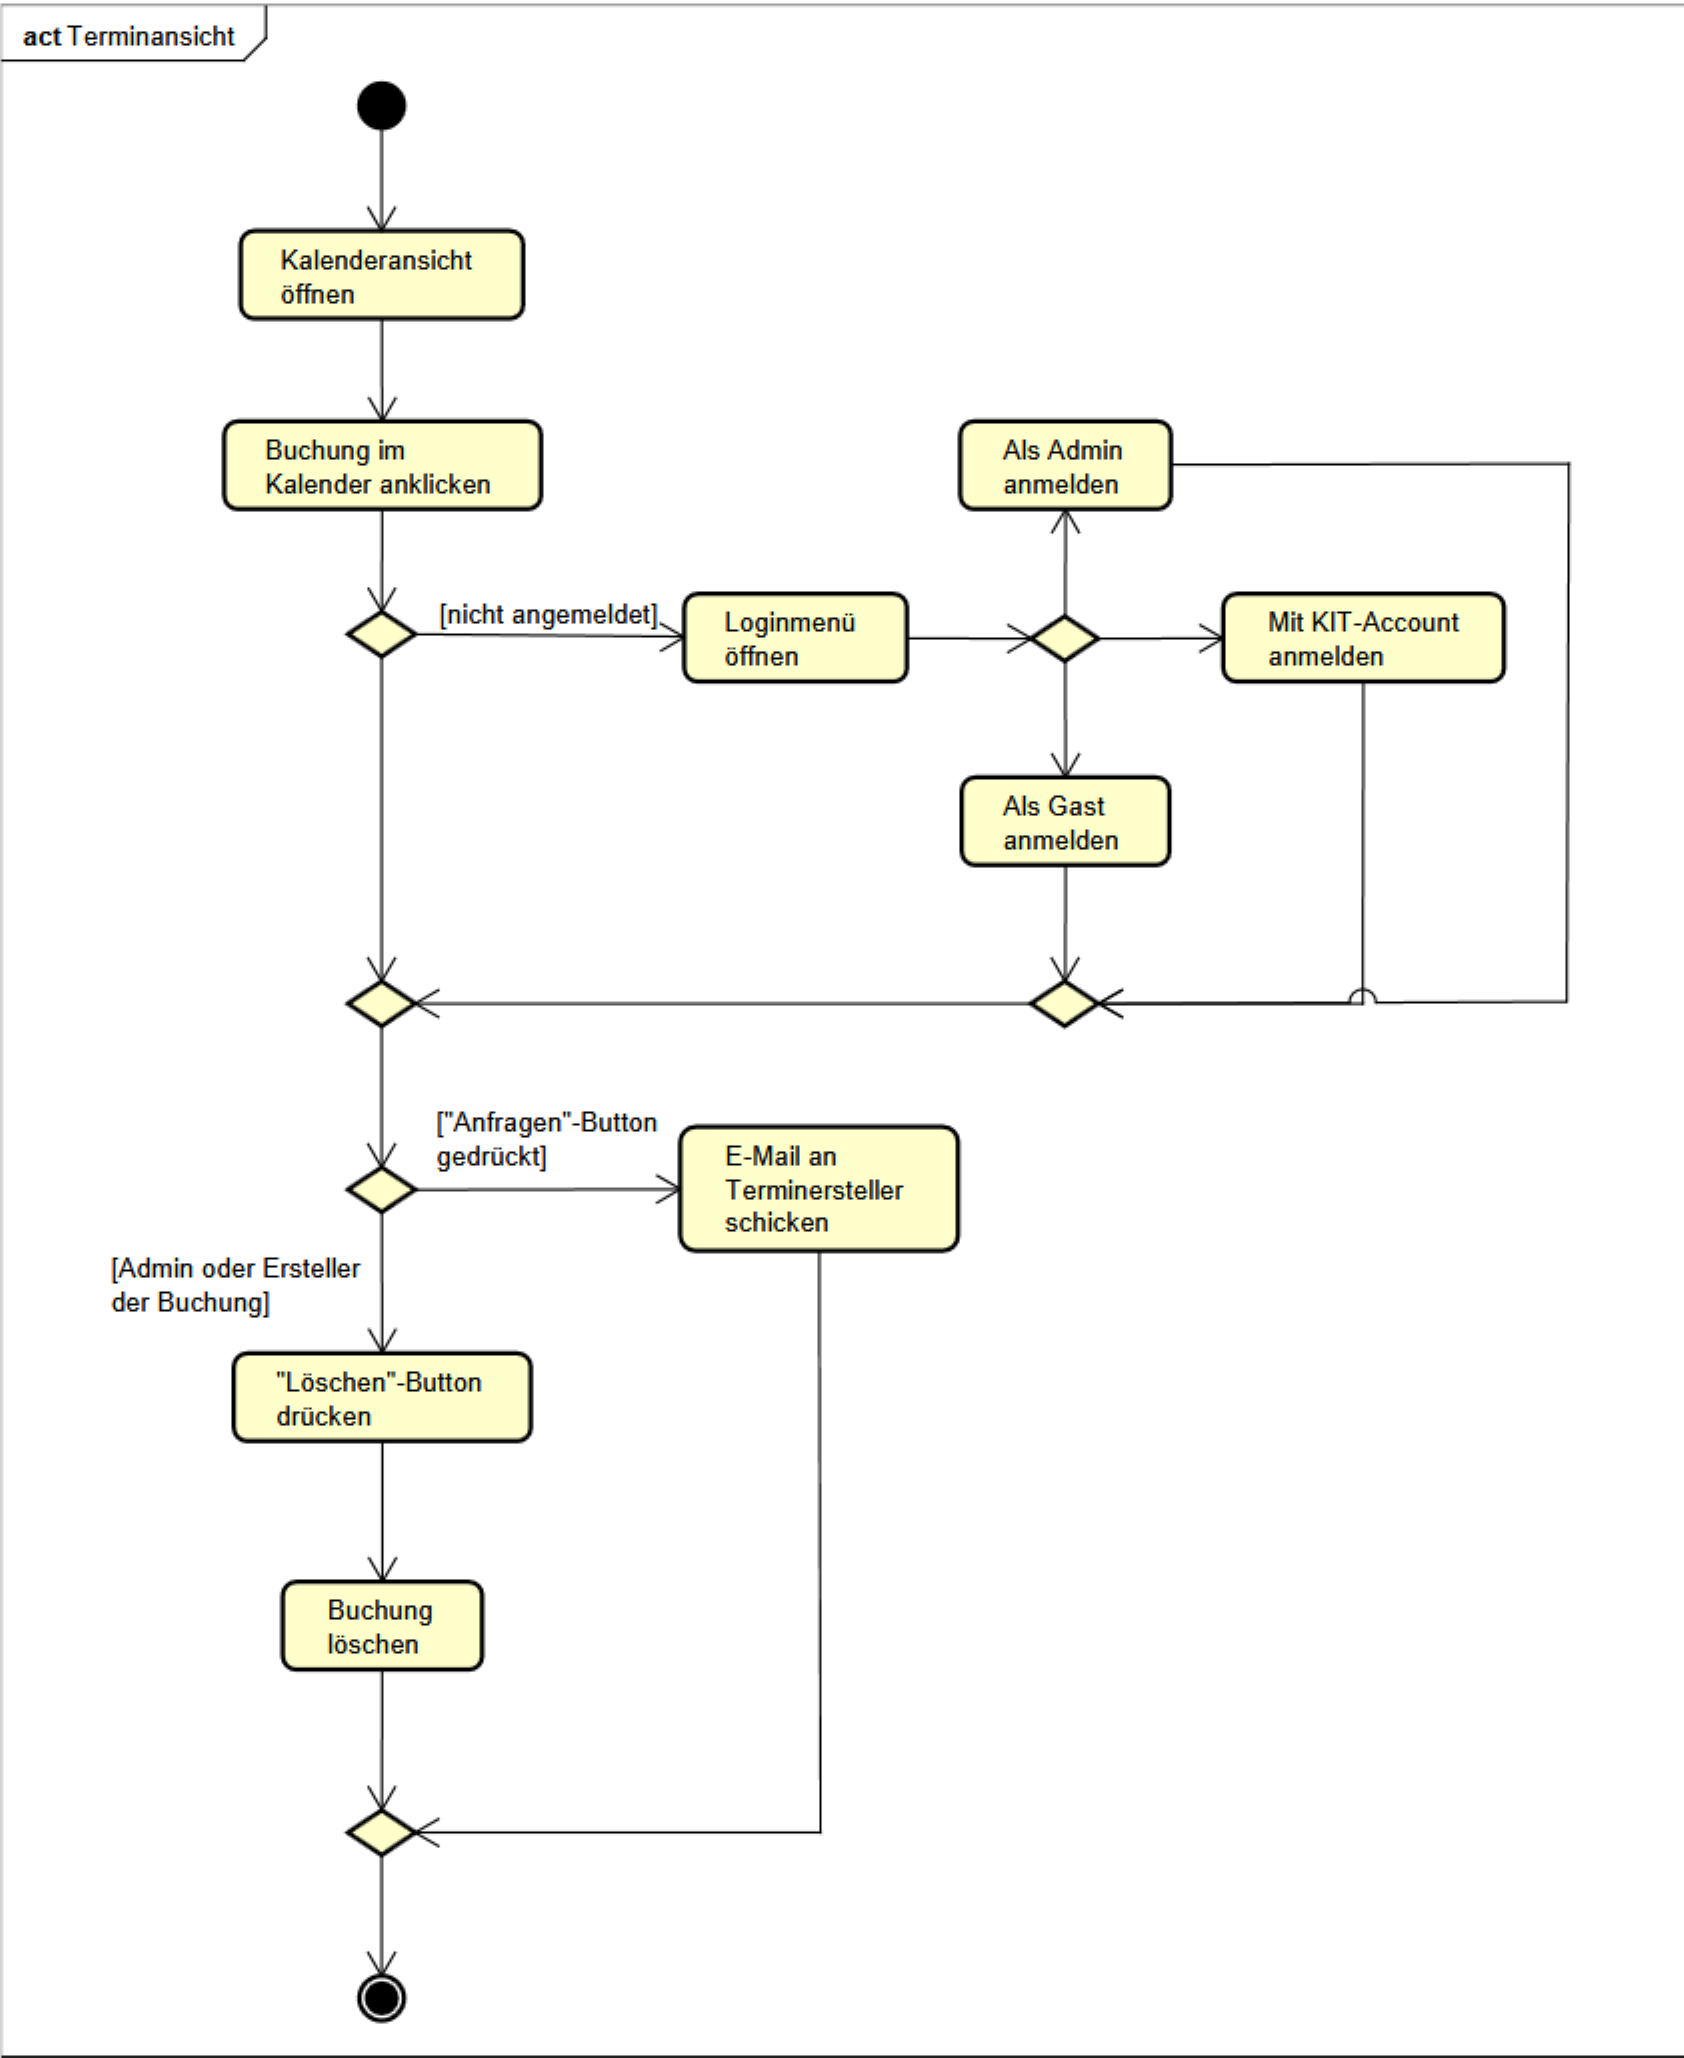
\includegraphics[width=\textwidth]{pictures/figures/activity/terminansicht}
        \label{fig:terminansichtprozess}
    \end{figure}
\end{frame}

\subsection{Checkout}
\begin{frame}{Checkout}
    \begin{figure}
        \leftfig
        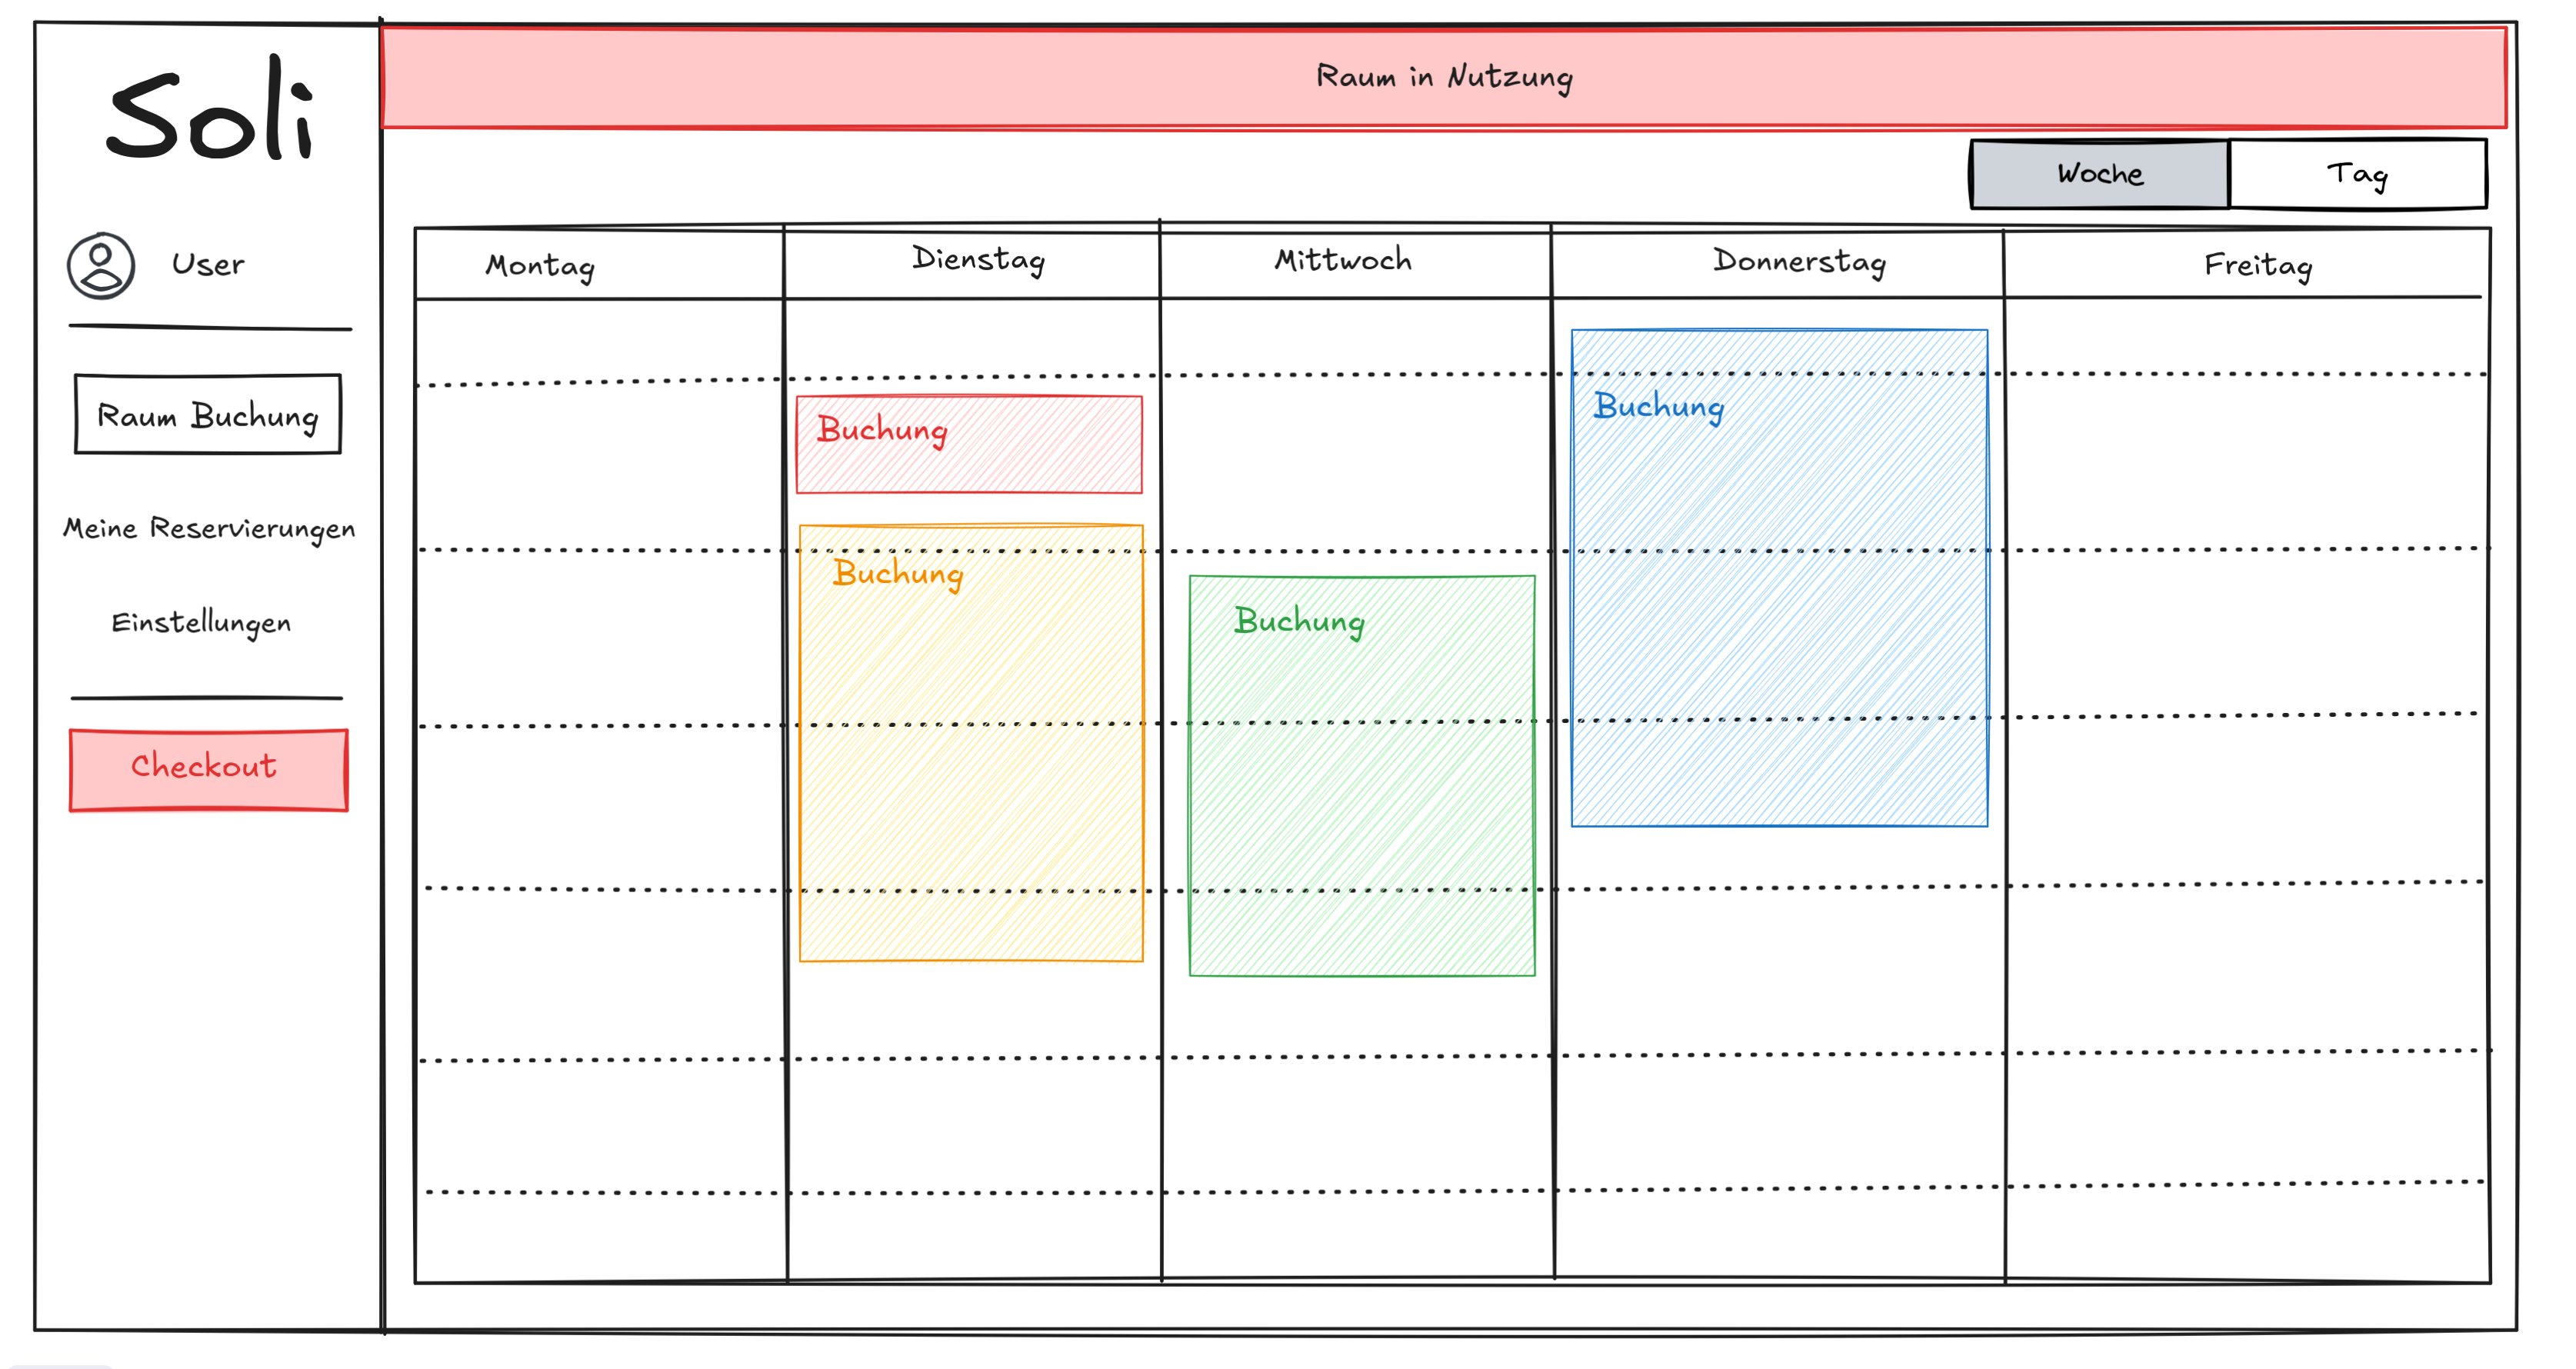
\includegraphics[width=\textwidth]{pictures/figures/ui/checkout}
        \label{fig:checkout}
    \end{figure}
    \begin{figure}
        \rightfig
        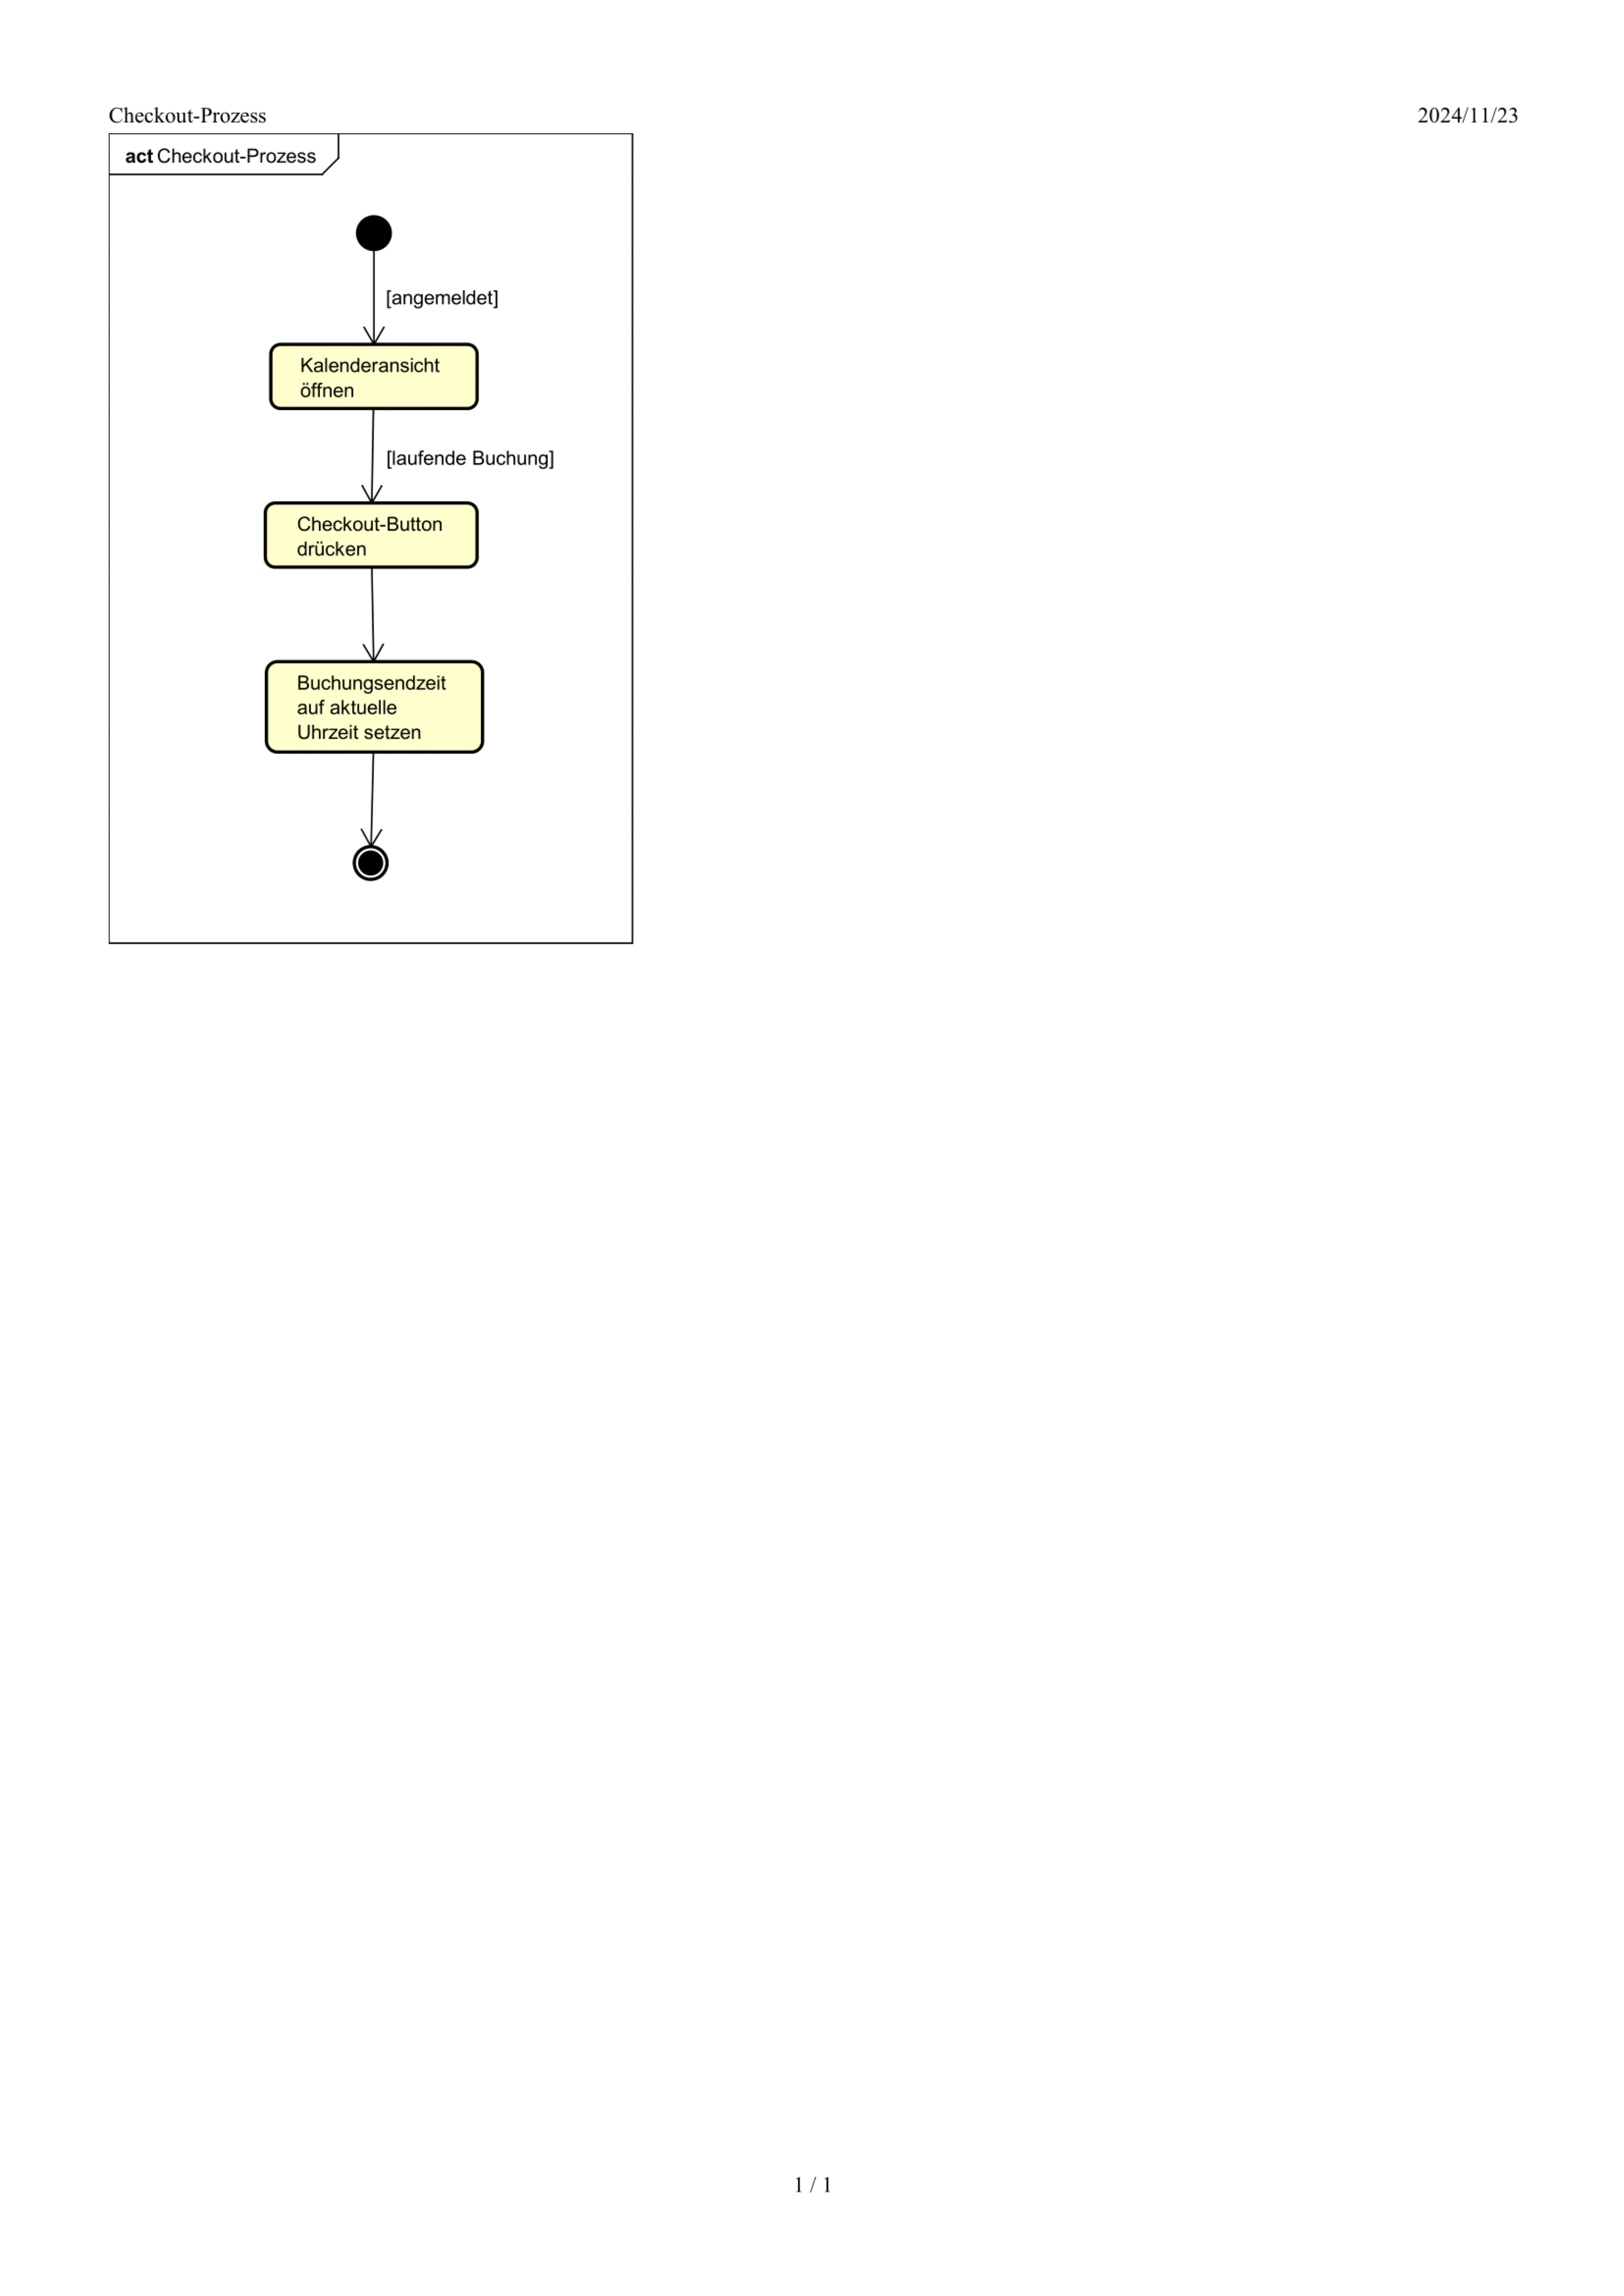
\includegraphics[width=\textwidth]{pictures/figures/activity/checkoutprozess} % TODO Bild anpassen
        \label{fig:checkoutprozess}
    \end{figure}
\end{frame}

\subsection{Kontenliste}
\begin{frame}{Kontenliste}
    \begin{figure}
        \centering
        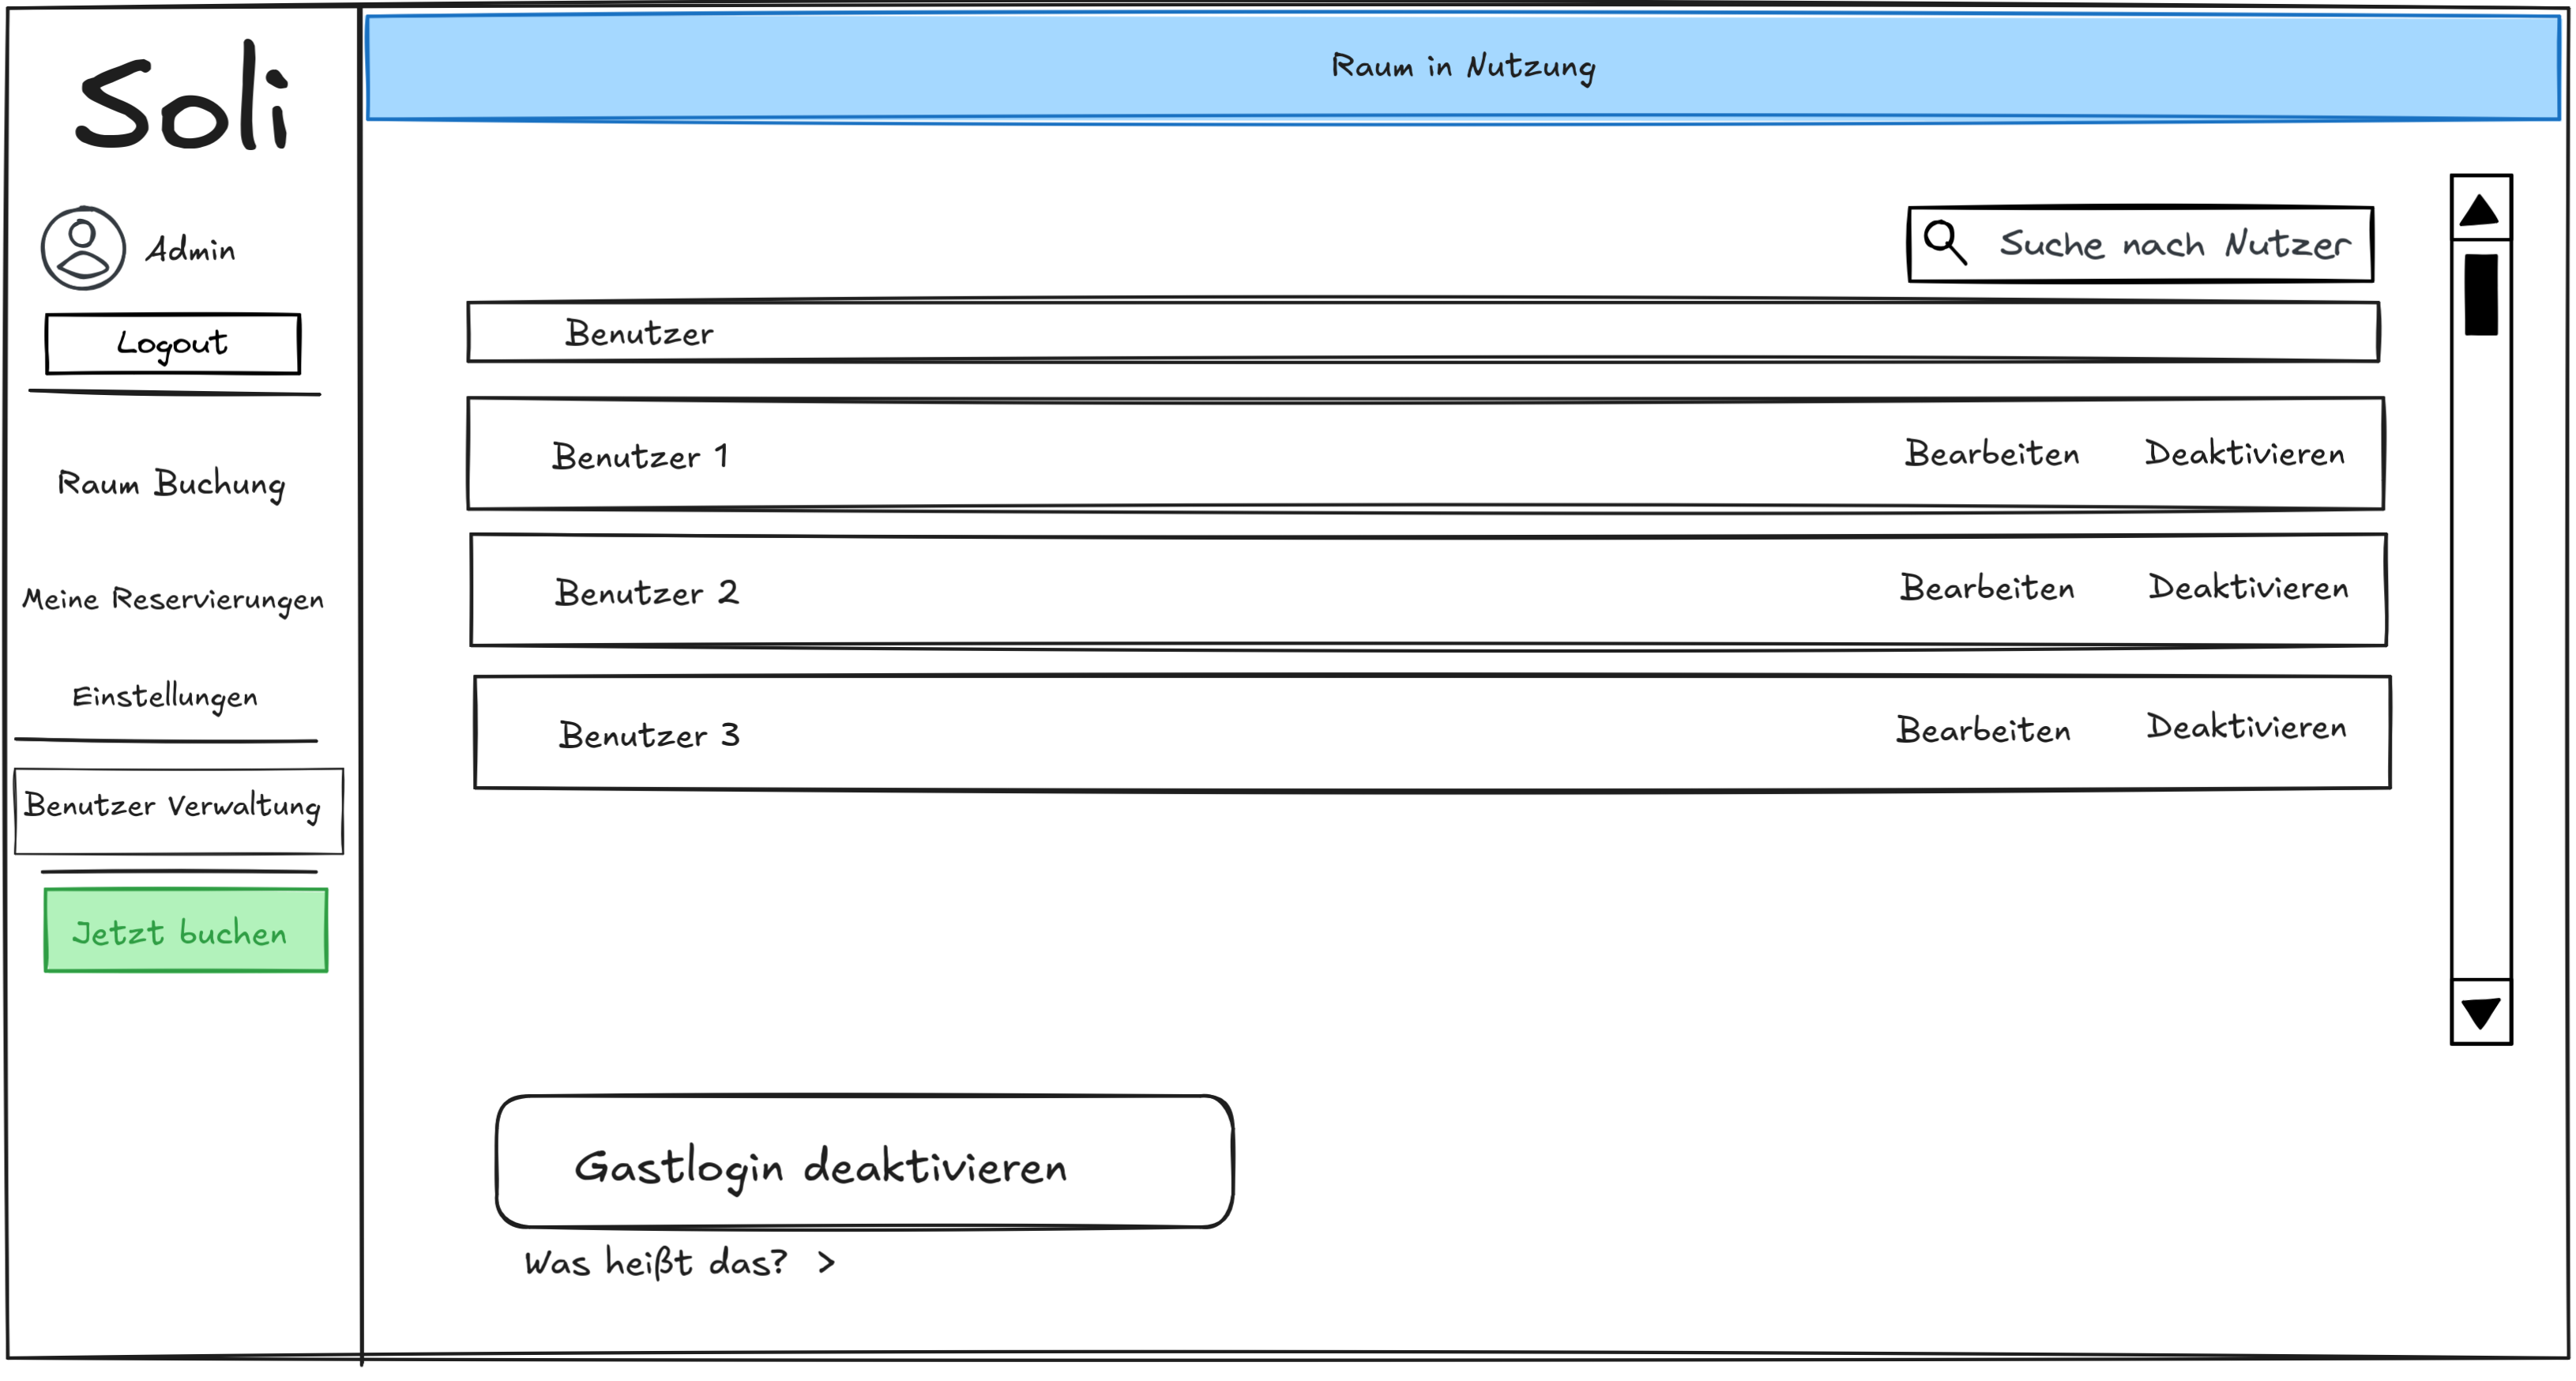
\includegraphics[width=\textwidth]{pictures/figures/ui/useradminui}
        \caption{Nur für Admins zugänglich.}
        \label{fig:kontenliste}
    \end{figure}
\end{frame}

\subsubsection{Adminfunktionalität}
\begin{frame}{Adminfunktionalität}
    \begin{figure}
        \centering
        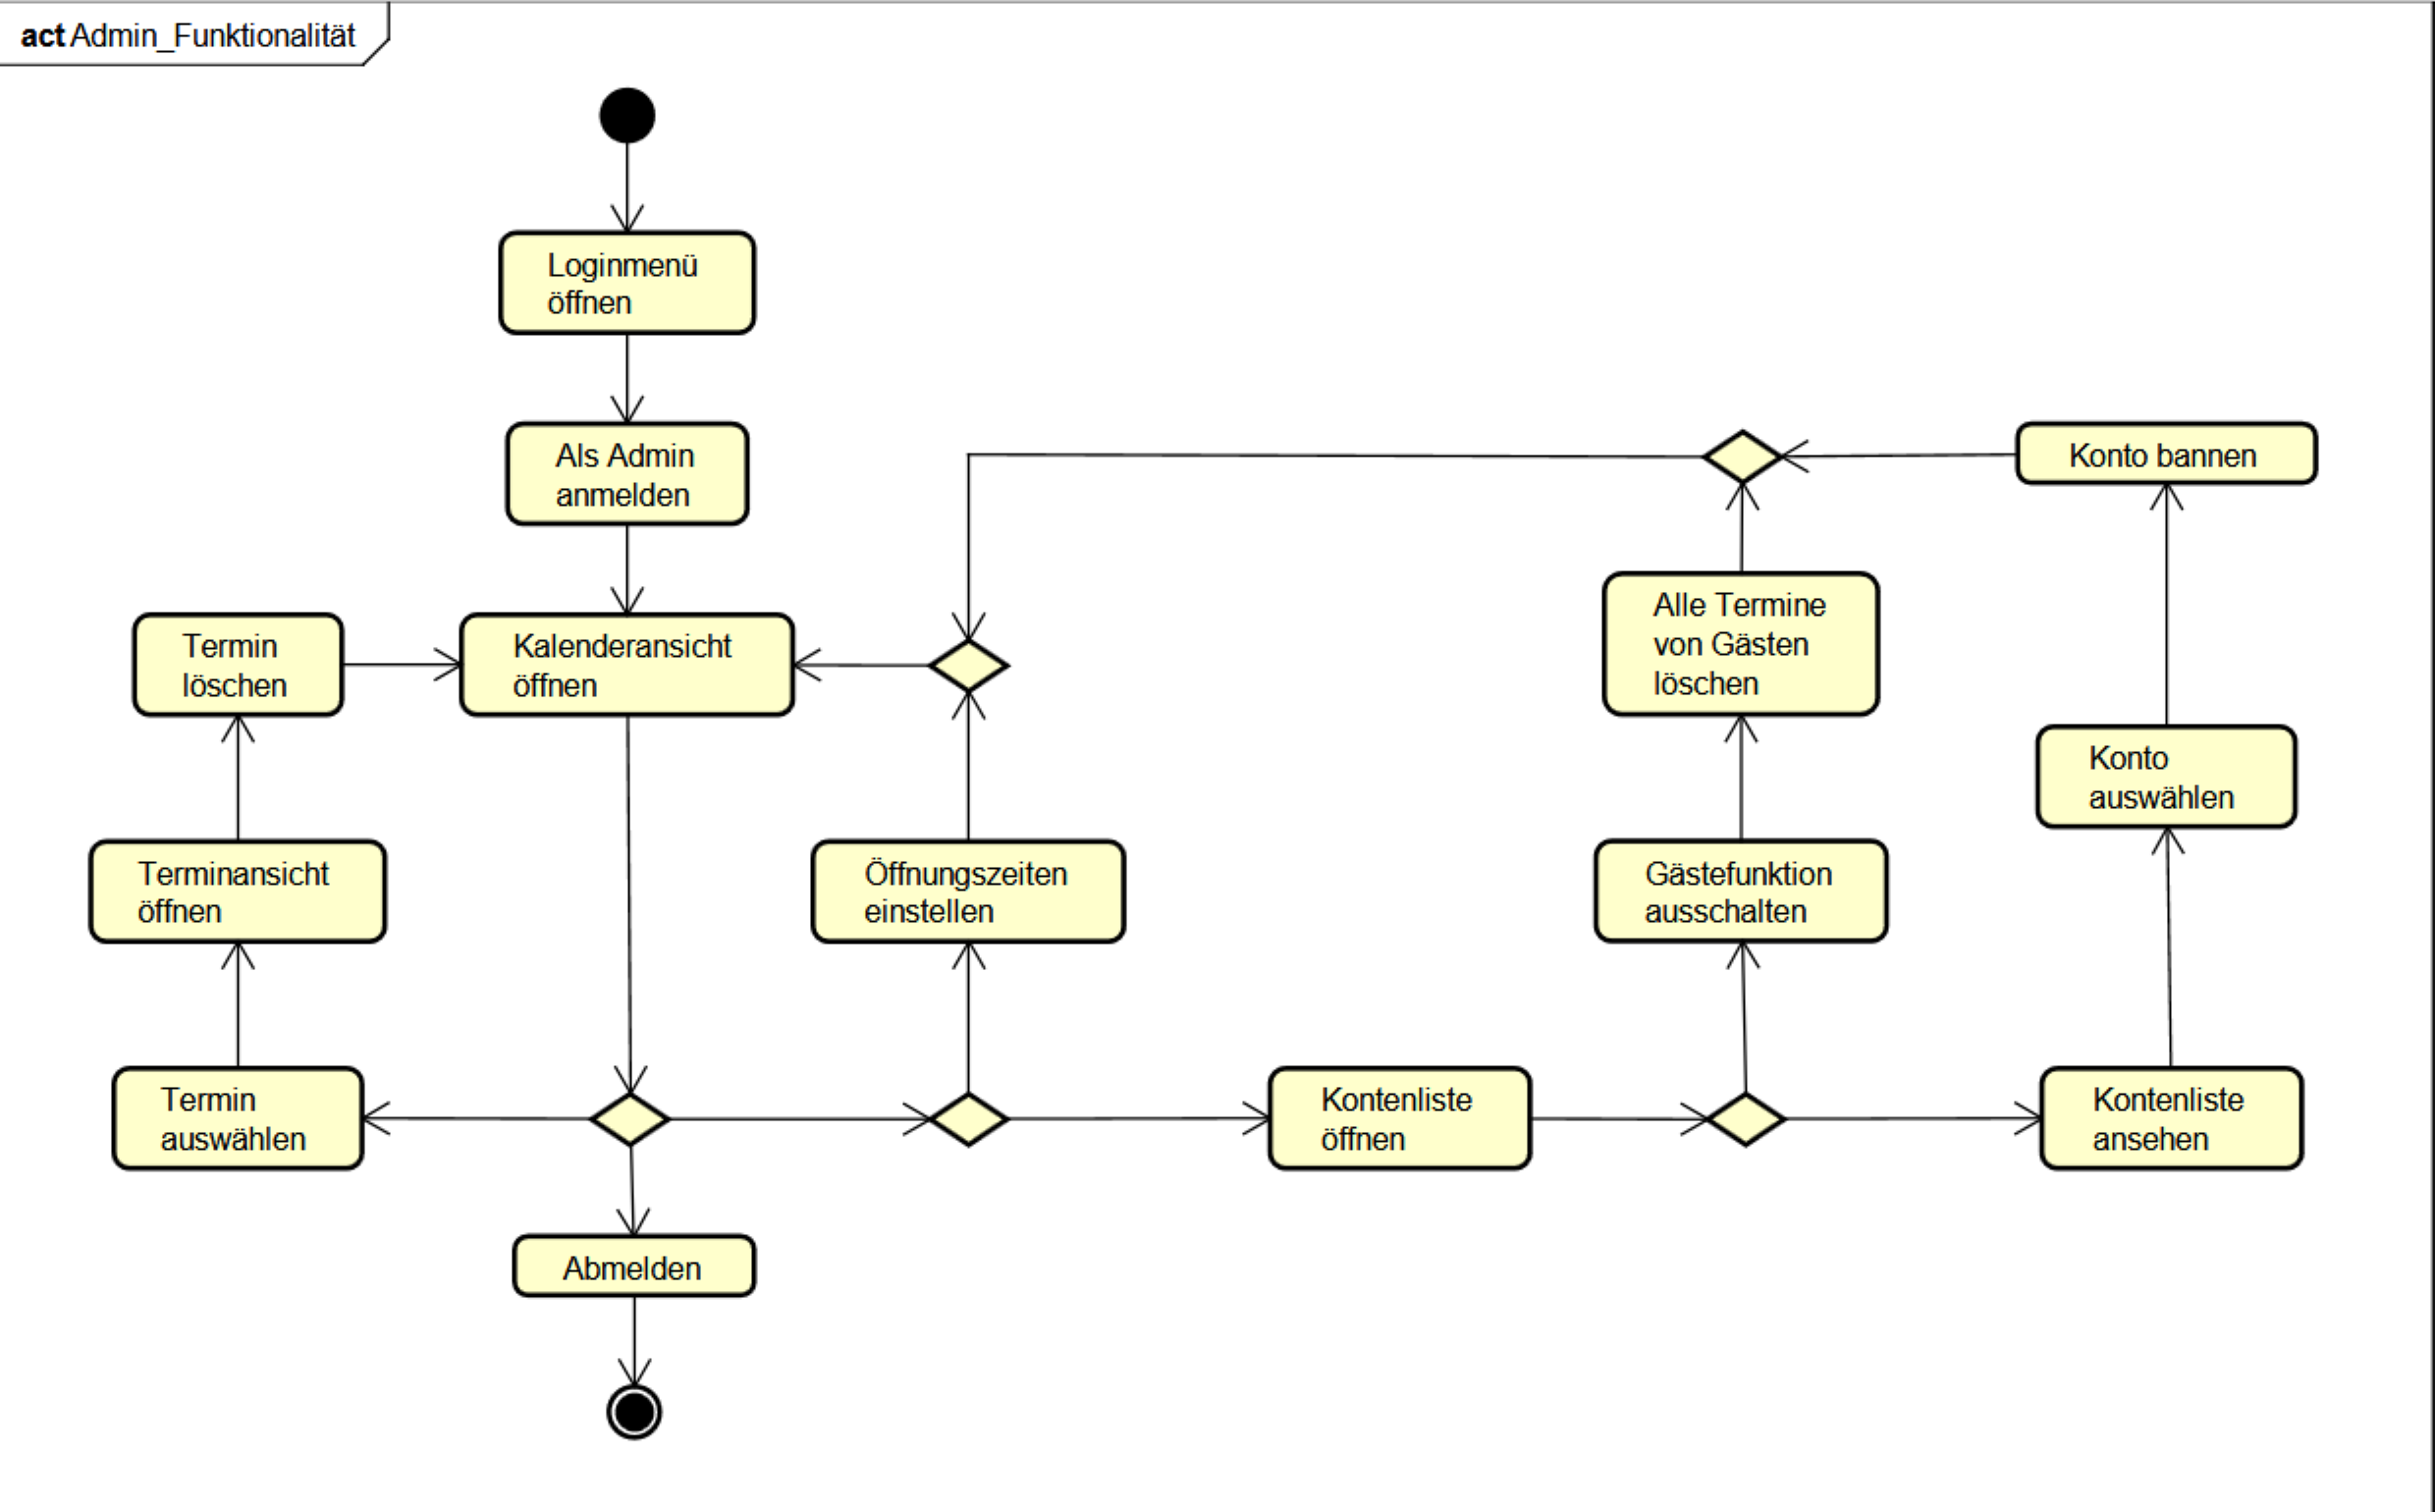
\includegraphics[width=\textwidth]{pictures/figures/activity/adminfunk}
        \label{fig:adminfunktionalitaet}
    \end{figure}
\end{frame}

% TODO Kaptitel Controller und der Rest

\end{document}